\documentclass{tietreport}

% Import images
\usepackage{graphicx}
\graphicspath{{figures/}}

% Tables, lists, floats, algorithm
\usepackage{booktabs}
\usepackage{tabularx}
\usepackage{array}
\usepackage{float}
\usepackage{enumitem}
\usepackage{subcaption}
\usepackage{algorithm}
\usepackage{algpseudocode}

% Bibliography configuration (as in the TIET template)
\usepackage[
  date=year,
  style=alphabetic,
  backend=biber,
  sorting=nty,
  maxnames=5,
  minnames=3,
  maxalphanames=4,
  minalphanames=3,
  backref=true,
  doi=false,
  isbn=false,
  url=true,
  eprint=false
]{biblatex}
\addbibresource{references.bib}

\newcolumntype{L}{>{\raggedright\arraybackslash}X}

%% ==================================================
%% TITLE PAGE
%% ==================================================

\TitlePageHeader{%
  UCS503P Software Engineering Lab: Project Report%
}

\ProjectTitle{%
  CampusSwap%
}

\ProjectSubTitle{%
  Room-Exchange and Slot-Coordination System for Campus\\[0.2cm]
  Prototype-stage report: multi-way hostel room swaps
  with Top Trading Cycles%
}

\author{%
  \texttt{1024240152} Jahnavi \\
  \texttt{1024240102} Ronit Saini \\
  \texttt{1024240001} Ranvir \\
  \texttt{1024240010} Krishna Kapoor%
}

\TitlePageSubText{%
  BE Third Year, 2026--27%
}

\AdvisorName{%
  Dr. Raghav B. Venkataramaiyer%
}

\TitlePageFooterText{{%
    \large Mid-Semester Evaluation (Prototype Stage) \\[0.2cm]
    \bfseries Computer Science and Engineering
    Department%
  } \\[0.15cm]
  Thapar Institute of Engineering and Technology,
  Patiala%
}

%% ==================================================

\begin{document}

\maketitle

\tableofcontents

% =====================================================
\chapter{Introduction}
% =====================================================

\section{Background and Motivation}

Hostel rooms at a university are allocated once, at the start of
a semester, and are then rarely changed. Students who would like
to move, for example to a lower floor, a single room, or closer to
friends, can only do so by \emph{trading} with another student,
because hostels run close to full capacity. Today these trades
are arranged informally through WhatsApp groups, notice boards and
personal contacts, and are approved on paper by the hostel office.

This project, \textbf{CampusSwap}, replaces that informal process
with a software workflow. Students submit a ranked list of rooms
they would prefer; the system finds \emph{chains} of exchanges in
which every participant moves to a room they prefer; every
participant confirms; and the warden approves. The matching step
uses the \textbf{Top Trading Cycles} (TTC) algorithm
of Shapley and Scarf~\cite{shapley1974cores}, which is the standard
method for markets in which each participant already owns one
indivisible good~\cite{abdulkadiroglu1999house}.

\section{Problem Statement}

The current process has four bottlenecks, identified in our
proposal:

\begin{itemize}
  \item \textbf{Fragmented information:} requests are scattered
    across chat groups and notice boards, so open offers are hard
    to find.
  \item \textbf{Search friction:} people look only for direct 1:1
    swaps (A with B). Multi-way chains such as
    A~$\rightarrow$~B~$\rightarrow$~C~$\rightarrow$~A satisfy everyone
    without needing an empty room, but are almost impossible to find
    by hand.
  \item \textbf{Administrative overhead:} approved swaps need paper
    applications and manual approval, with no central record.
  \item \textbf{No visibility:} applicants cannot tell whether a
    match is pending, being processed, or impossible.
\end{itemize}

Finding such chains is a graph-search problem, which makes it well
suited to a software solution.

\section{Objectives}

The proposal defined Phase~1 success as \emph{accepting a request,
persisting it to the database, executing a match, and rendering
the result}. The objectives for this prototype stage were:

\begin{enumerate}
  \item \textbf{O1 -- Data model:} a relational schema for hostels,
    rooms, beds, students, requests and matches.
  \item \textbf{O2 -- Student module:} authentication and ranked
    preference entry (up to five rooms) with full validation.
  \item \textbf{O3 -- Matching engine:} a TTC implementation backed
    by unit tests on synthetic data.
  \item \textbf{O4 -- Dashboards and CI:} a student status dashboard,
    an administrator console, and continuous integration that runs
    the tests on every change.
  \item \textbf{O5 -- Evaluation:} measure Match Yield (MY), the
    percentage of students placed in an exchange chain, against the
    target MY~$\geq 60\%$ for 100 requests, and compare with direct
    1:1 swaps only.
\end{enumerate}

Chapter~\ref{ch:eval} reports whether each objective was met.

\section{Scope of the Prototype}

\textbf{Included:} student and hostel-staff login; room browsing
and ranked requests (feature~1); TTC matching rounds with a dry-run
mode and a TTC-versus-1:1 comparison (feature~2); the multi-party
confirmation workflow with a 48-hour deadline, which the proposal
planned for Phase~2; warden approval; CSV export; an audit log.

\textbf{Not included yet:} the institute single sign-on, e-mail
notifications, the PDF sign-off form, the faculty slot-exchange
module, and deployment to a public server. All data used in this
report is synthetic.

% =====================================================
\chapter{Requirements and Design}
% =====================================================

\section{Users and Use Cases}

Two kinds of people use the system: \textbf{students}, who submit,
withdraw, confirm or decline swaps, and \textbf{hostel staff (the
warden)}, who run matching rounds and approve swaps.
Figure~\ref{fig:usecase} shows the use cases.

\begin{figure}[H]
  \centering
  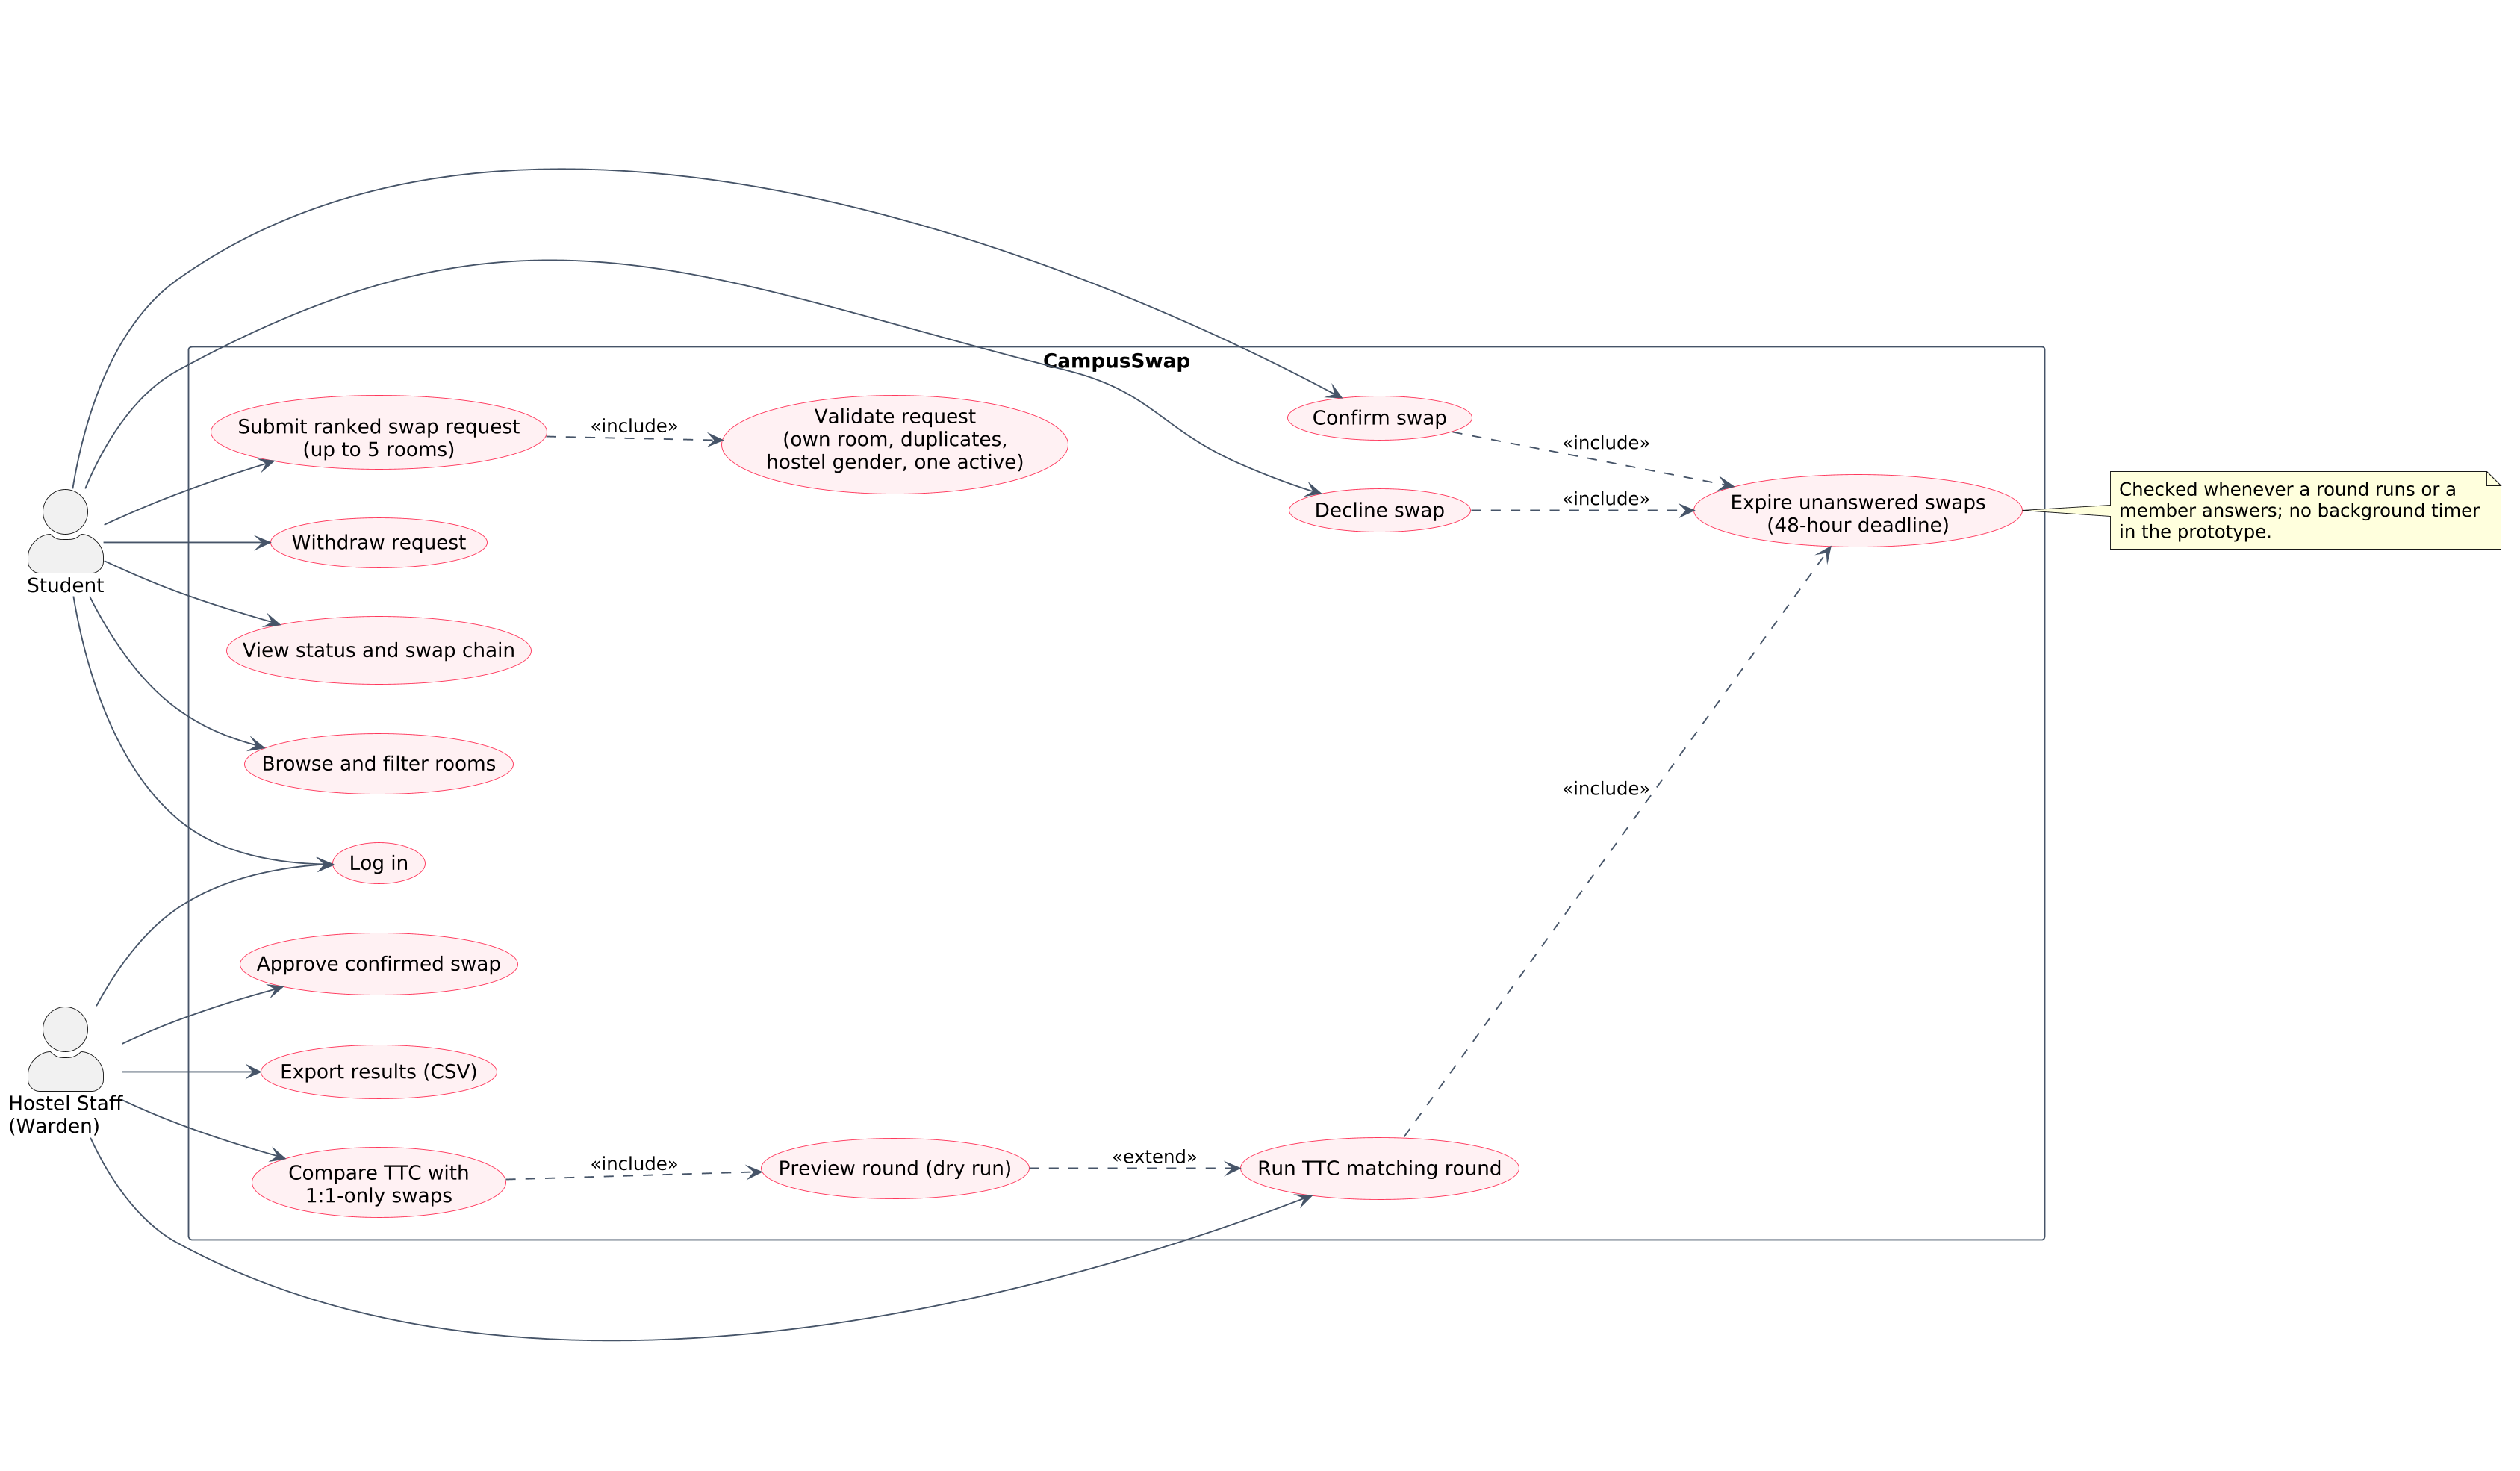
\includegraphics[width=\textwidth]{use-case.png}
  \caption{Use Case diagram of the prototype.}
  \label{fig:usecase}
\end{figure}

The relationships in the diagram are justified as follows:
\begin{itemize}
  \item \emph{Submit ranked request} $\langle\langle$include$\rangle\rangle$
    \emph{Validate request}: validation is a mandatory part of every
    submission.
  \item \emph{Run matching round}, \emph{Confirm swap} and \emph{Decline swap}
    $\langle\langle$include$\rangle\rangle$ \emph{Expire unanswered swaps}:
    each of them first dissolves chains whose 48-hour deadline has passed.
  \item \emph{Preview round (dry run)} $\langle\langle$extend$\rangle\rangle$
    \emph{Run matching round}: an optional variation chosen by the warden.
  \item \emph{Compare TTC with 1:1 swaps} $\langle\langle$include$\rangle\rangle$
    \emph{Preview round}: a comparison always runs both algorithms as dry runs.
\end{itemize}
There is no clock actor: in the prototype the deadline is checked
whenever something happens, not by a background timer.

\section{Functional Requirements}

\begin{table}[H]
\centering
\begin{tabularx}{\textwidth}{@{}lL@{}}
\toprule
\textbf{ID} & \textbf{Requirement} \\
\midrule
FR1 & Students and staff log in with an institute e-mail and password; each role sees only its own pages and API endpoints. \\
FR2 & A student can browse rooms only in hostels they are allowed to live in, filtered by hostel, floor, type, AC and washroom. \\
FR3 & A student submits 1--5 ranked rooms; the system rejects duplicates, their own room, unknown rooms, the other gender's hostels, and a second active request. Each request receives a tracking ID. \\
FR4 & A student can withdraw a request while it is still in the pool. \\
FR5 & The warden runs a TTC round over all open requests; the result is stored with a readable round-by-round trace. \\
FR6 & The warden can preview a round without saving it, and compare TTC with direct 1:1 swaps on the same pool. \\
FR7 & Every member of a proposed chain confirms or declines within 48 hours; one decline or a missed deadline cancels the chain and returns the others to the pool. \\
FR8 & The warden approves a fully confirmed chain, after which the students' beds change hands. \\
FR9 & Every request, round, answer and approval is recorded in an audit log; all requests can be exported as CSV. \\
\bottomrule
\end{tabularx}
\caption{Functional requirements.}
\end{table}

\section{Non-Functional Requirements}

\begin{itemize}
  \item \textbf{Correctness:} every matching round is saved in one
    database transaction (all or nothing).
  \item \textbf{Security:} salted password hashes; session tokens in
    HttpOnly cookies with only their hash stored; server-side role
    checks; escaping of all user-supplied text in the pages.
  \item \textbf{Responsiveness:} pages work on phones and desktops.
  \item \textbf{Performance:} a matching round for a whole hostel
    completes well within one second.
  \item \textbf{Operability:} the prototype runs with one command and
    without internet access (fonts and styles are bundled).
\end{itemize}

\section{System Architecture}

CampusSwap is a three-tier web application with a separate matching
engine (Figure~\ref{fig:sequence} shows the tiers in action):

\begin{enumerate}
  \item \textbf{Presentation:} four HTML pages with small JavaScript
    modules that call a JSON API.
  \item \textbf{Application:} FastAPI routes~\cite{fastapi} that check the
    caller's session and role, and \emph{services} that contain every
    business rule.
  \item \textbf{Data:} a relational SQLite database accessed through
    SQLAlchemy~\cite{sqlalchemy}.
  \item \textbf{Engine:} a pure-Python TTC module with no database or
    web code, called by the matching service. It can therefore be
    unit-tested in isolation and reused for faculty slots later.
\end{enumerate}

\begin{table}[H]
\centering
\begin{tabularx}{\textwidth}{@{}lL@{}}
\toprule
\textbf{Layer} & \textbf{Technology} \\
\midrule
Frontend & HTML, JavaScript modules, Tailwind CSS 3.4 (built locally) \\
Backend & Python 3.12, FastAPI 0.141, Uvicorn \\
Database & SQLite through SQLAlchemy 2.0 (ACID transactions) \\
Testing and CI & pytest 9 (90 tests), GitHub Actions \\
Diagrams and docs & PlantUML~\cite{plantuml}, MkDocs on GitHub Pages \\
\bottomrule
\end{tabularx}
\caption{Technology stack.}
\end{table}

\section{Data Model}

Figure~\ref{fig:class} shows the classes. Key design decisions:

\begin{itemize}
  \item \textbf{Generalisation:} \texttt{Student} and \texttt{Admin}
    are kinds of \texttt{User}; both are stored in one table.
  \item \textbf{Composition:} a \texttt{Hostel} owns its
    \texttt{Room}s and a room owns its 1--3 \texttt{Seat}s (beds);
    a \texttt{SwapRequest} owns its 1--5 \texttt{Preference}s; a
    \texttt{MatchRun} owns its \texttt{SwapCycle}s, each with at least
    two \texttt{CycleMember}s.
  \item \textbf{Association:} a seat has at most one occupant and a
    student at most one seat. Students exist independently of seats,
    so this is an association rather than composition.
  \item \textbf{Why seats and not rooms:} in a double room only one of
    the two students moves, so the unit of exchange is a bed.
\end{itemize}

\begin{figure}[H]
  \centering
  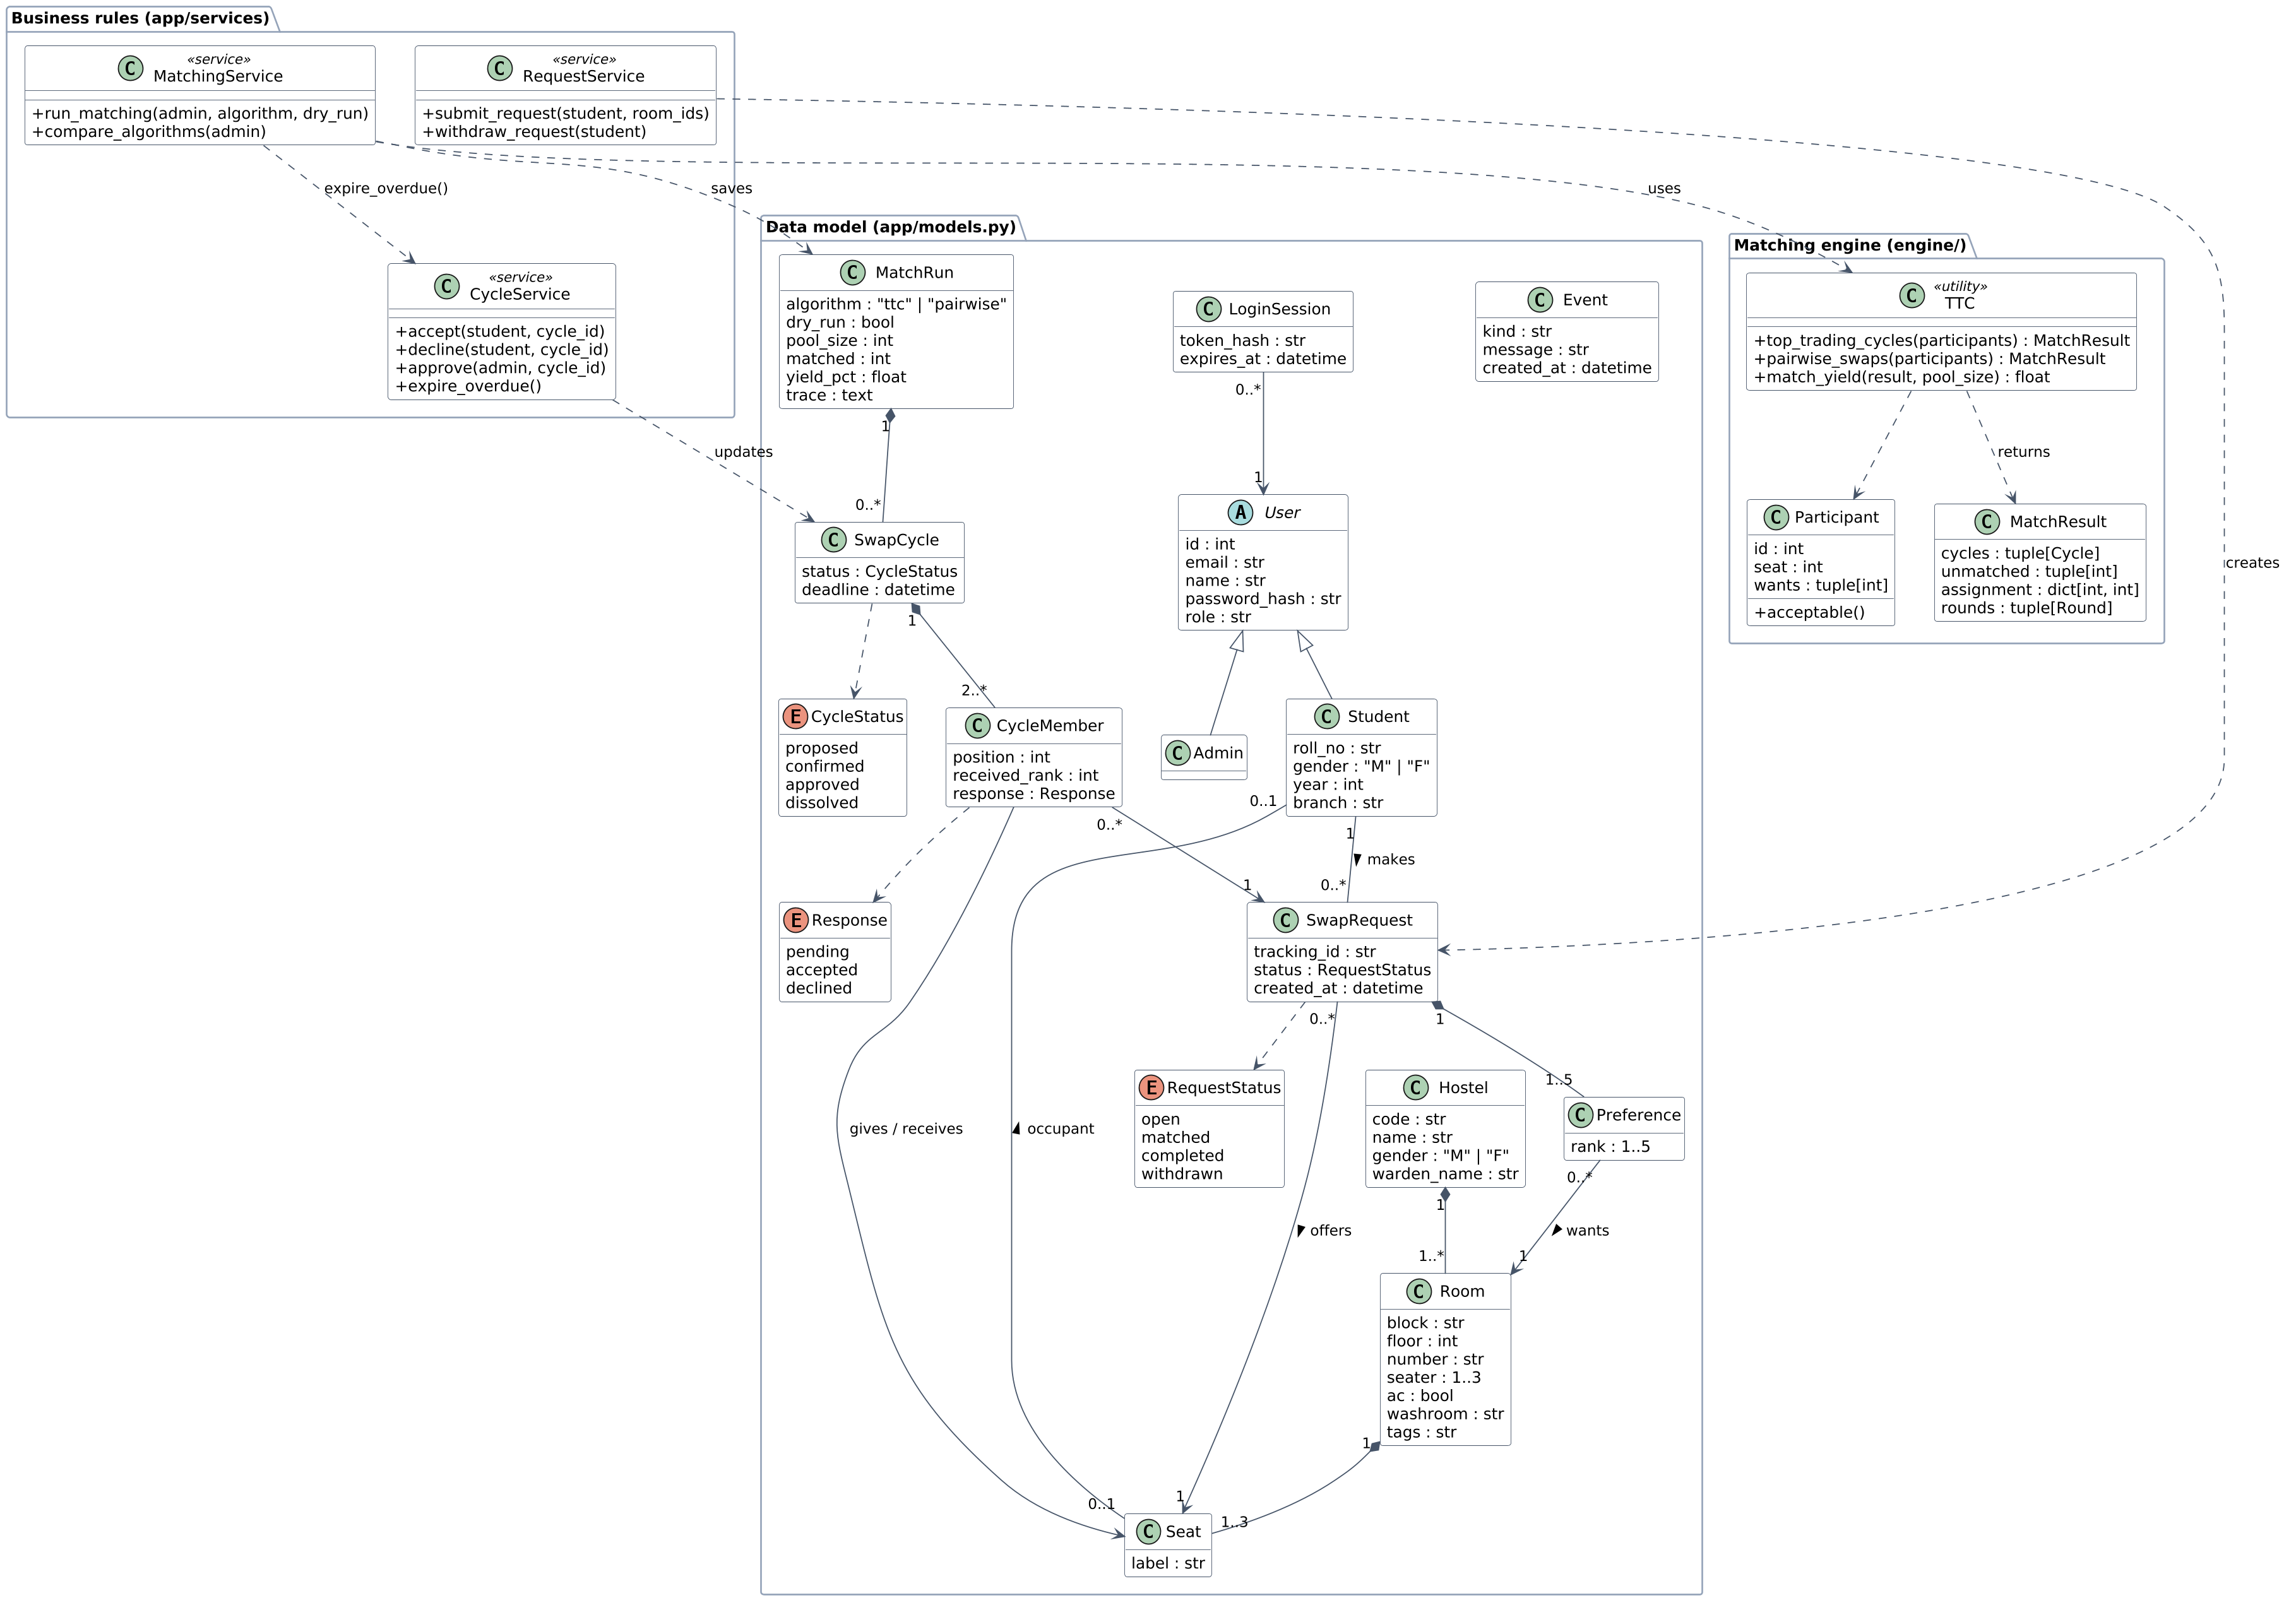
\includegraphics[width=\textwidth,height=0.8\textheight,keepaspectratio]{class.png}
  \caption{Class diagram: data model, services and engine.}
  \label{fig:class}
\end{figure}

\section{Behaviour}

Figure~\ref{fig:sequence} traces one swap from request to approval
through every layer, and Figure~\ref{fig:activity} shows the life of
a request, including the decline and deadline branches.

\begin{figure}[H]
  \centering
  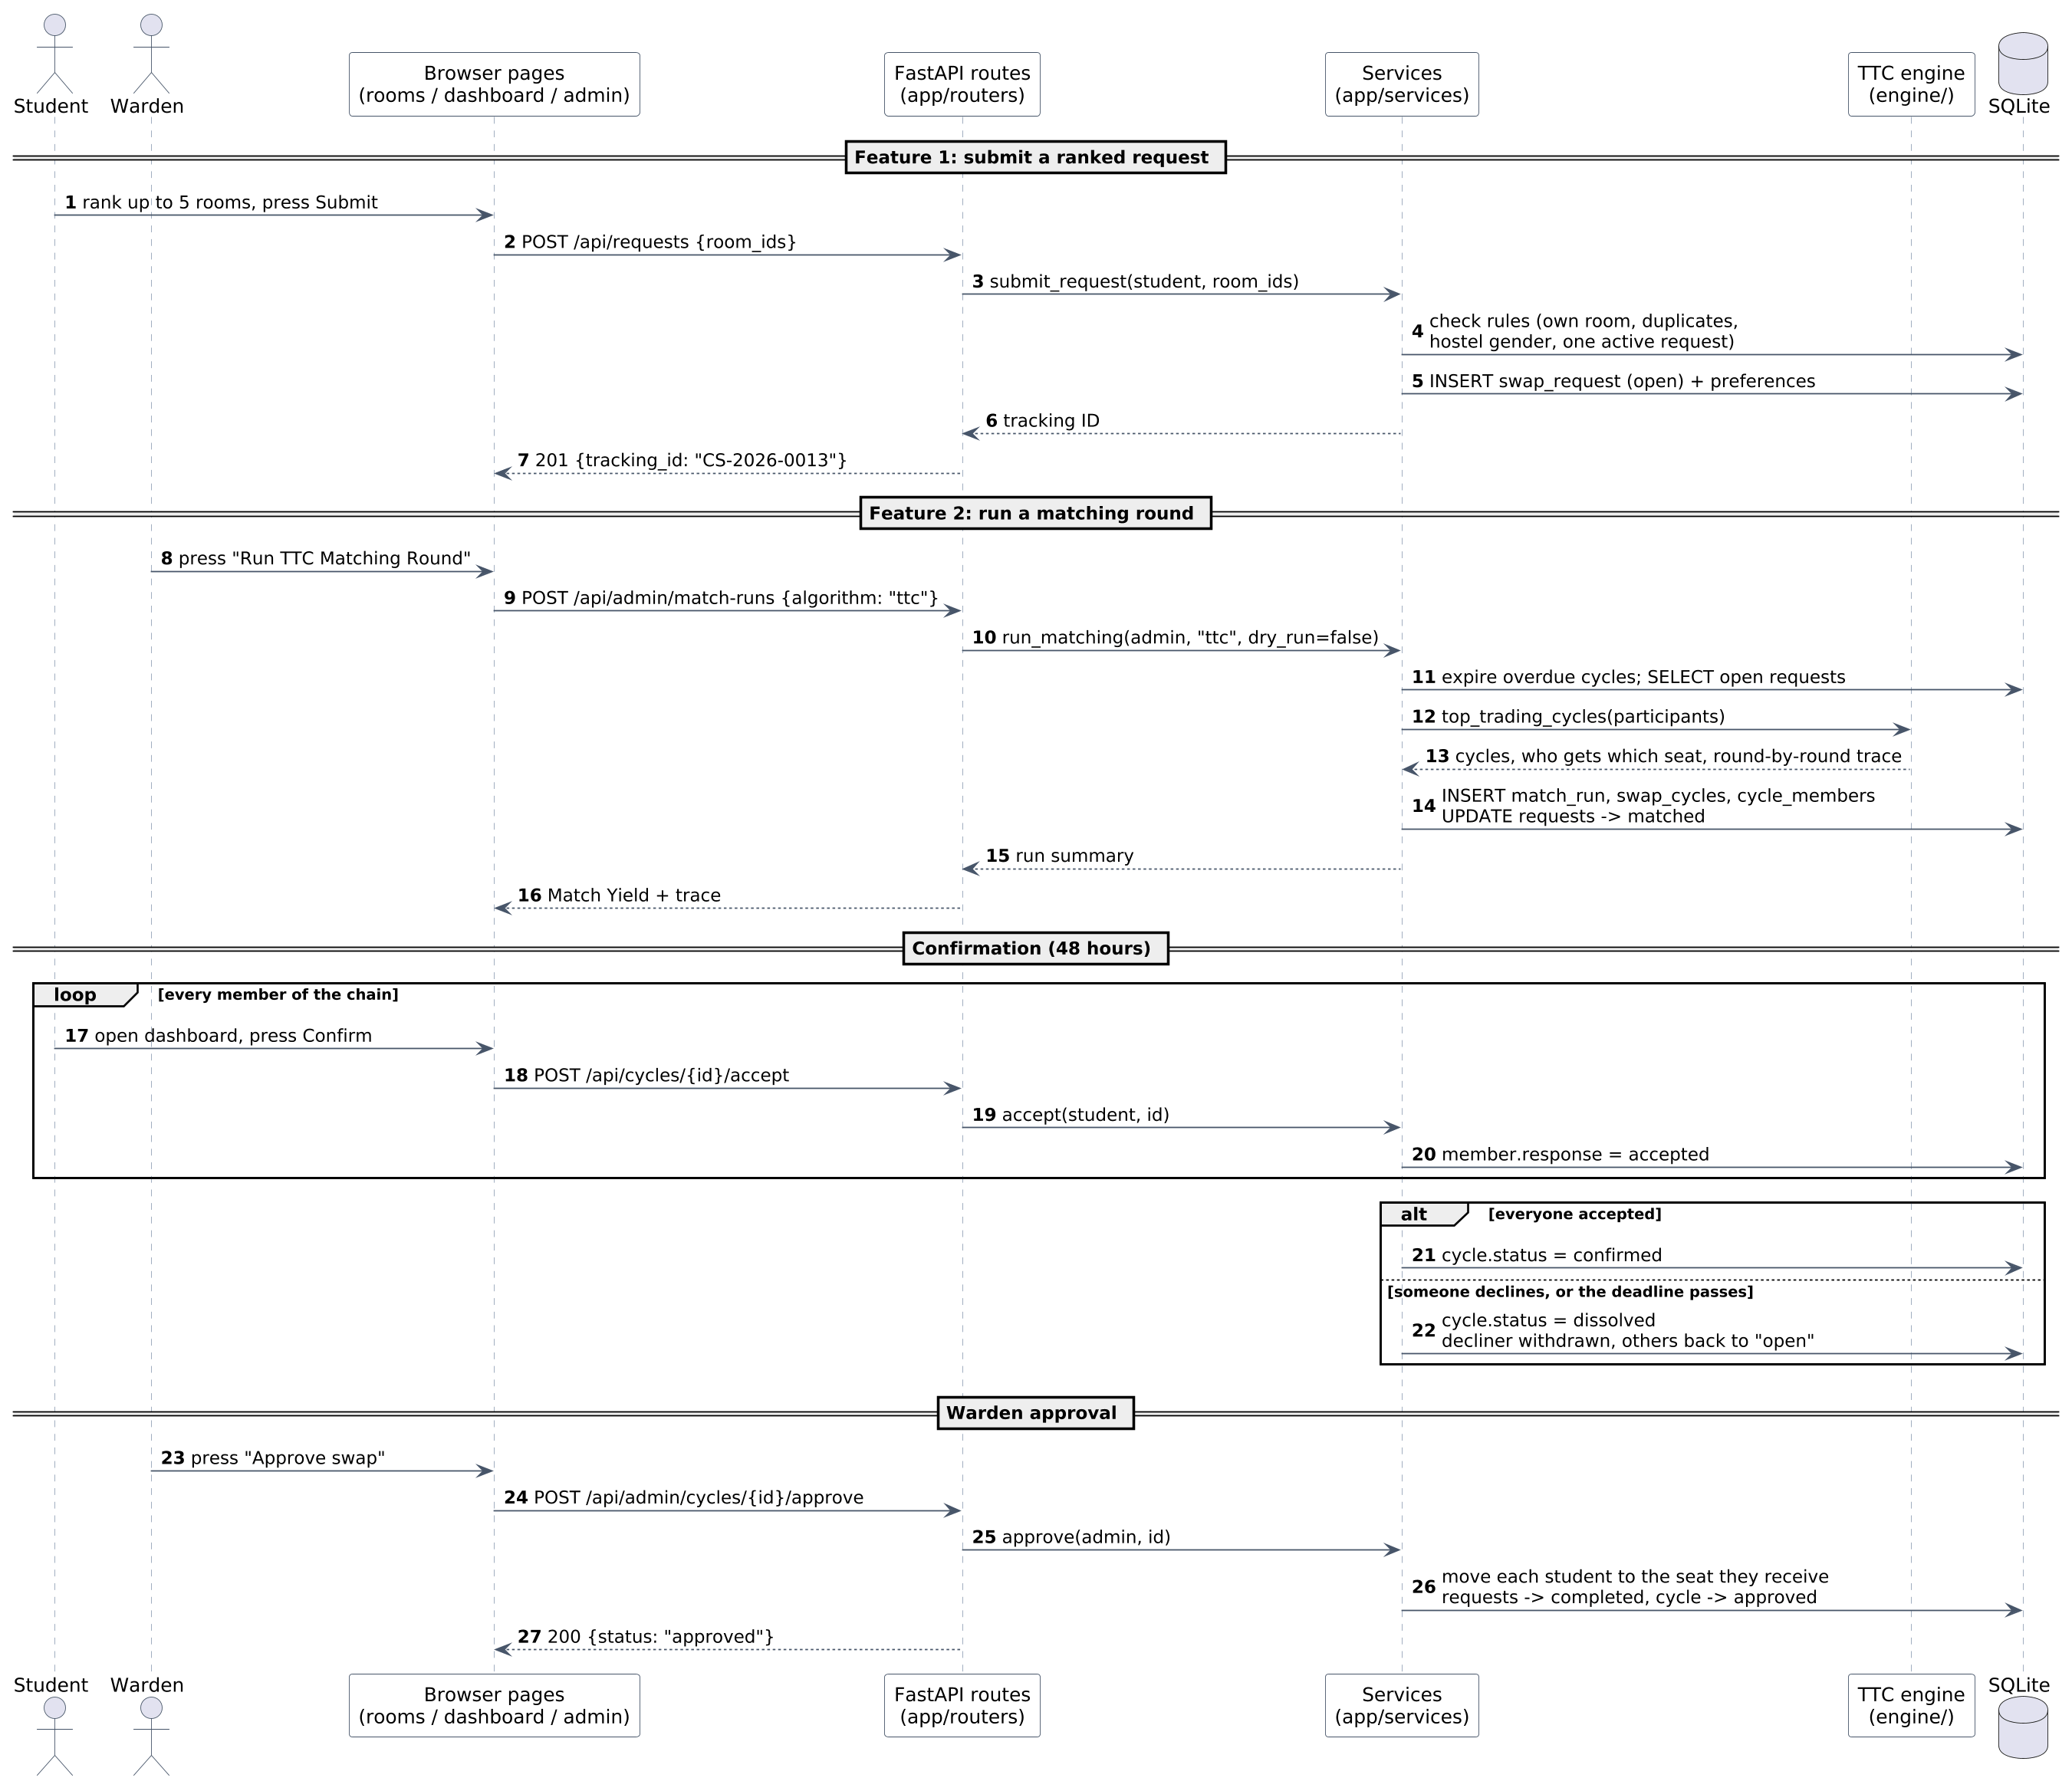
\includegraphics[width=\textwidth,height=0.8\textheight,keepaspectratio]{sequence.png}
  \caption{Sequence diagram: submit, match, confirm and approve.}
  \label{fig:sequence}
\end{figure}

\begin{figure}[H]
  \centering
  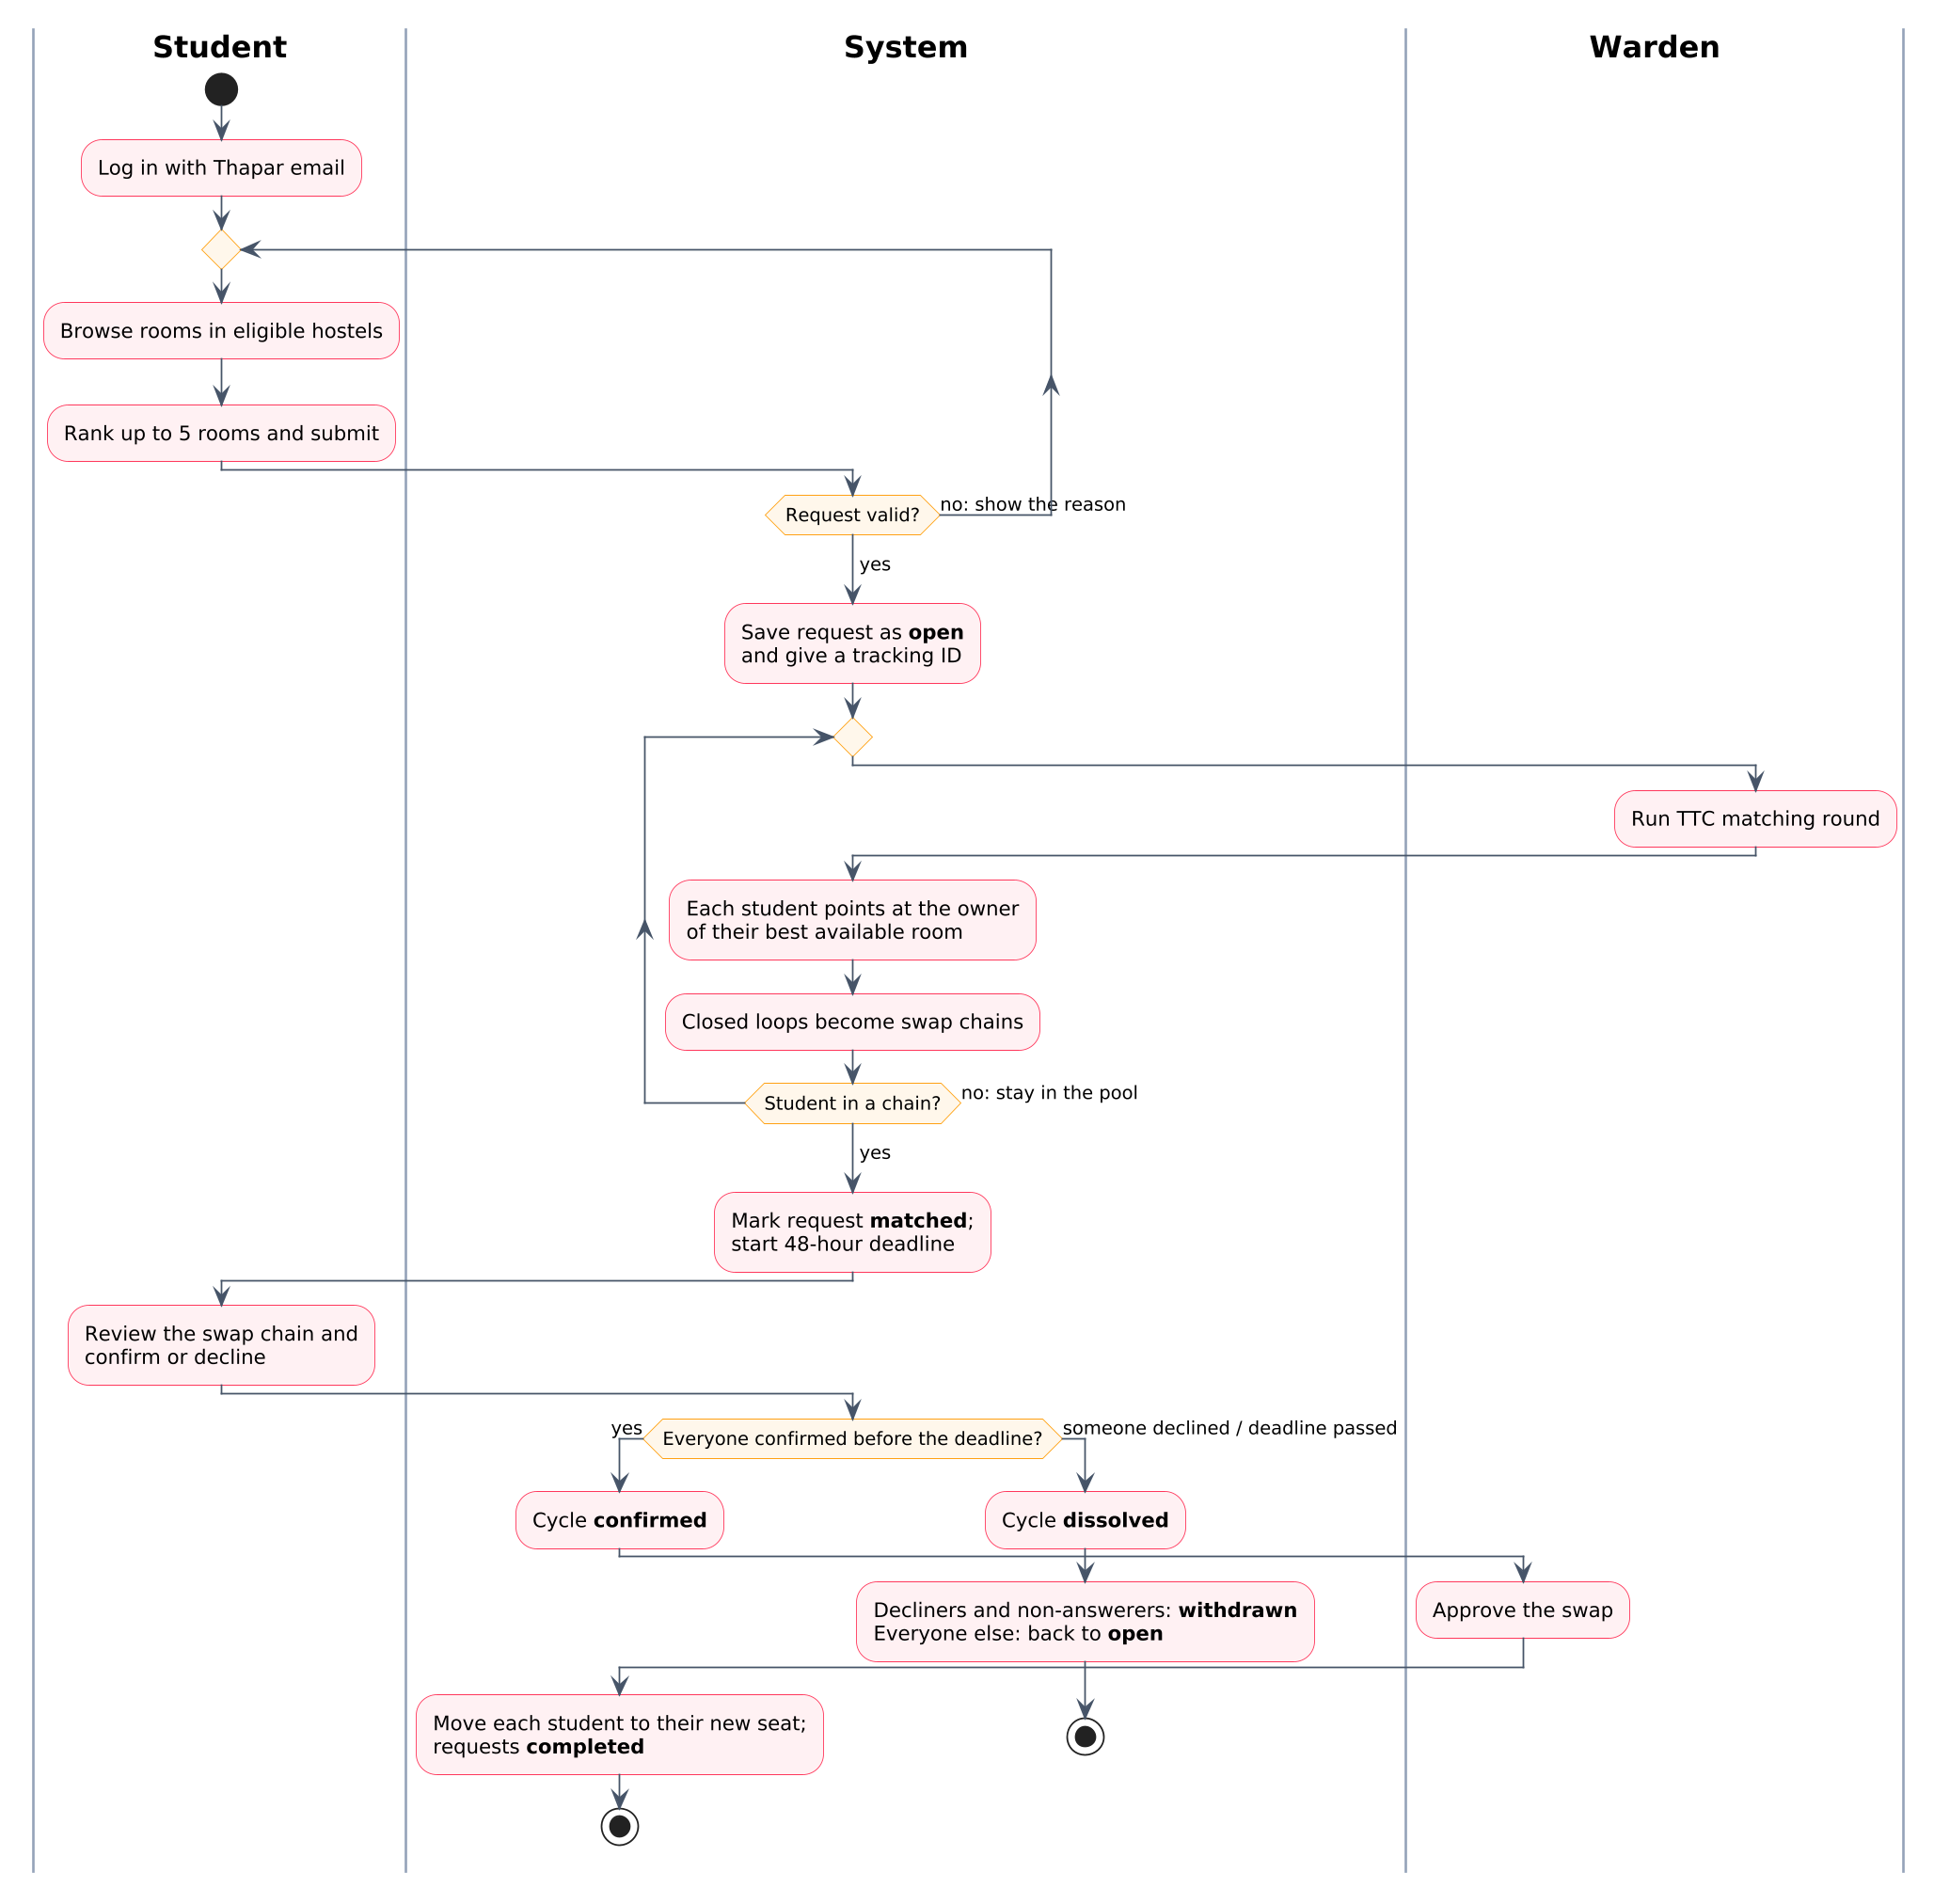
\includegraphics[width=\textwidth,height=0.8\textheight,keepaspectratio]{activity.png}
  \caption{Activity diagram: the life of a swap request.}
  \label{fig:activity}
\end{figure}

% =====================================================
\chapter{Implementation}
% =====================================================

\section{Matching Engine}

\subsection{Model}

Each open request becomes a \emph{participant} $p$ that owns one
seat $s_p$ and has a ranked list $w_p$ of seats it would accept.
Students rank \emph{rooms}; the service expands each room into its
seats in seat-ID order, so a double room can be obtained from either
occupant who is in the pool. Seats listed after the participant's own
seat count as worse than staying.

\subsection{Top Trading Cycles}

Algorithm~\ref{alg:ttc} is implemented in
\texttt{code/backend/engine/ttc.py}.

\begin{algorithm}[H]
\caption{Top Trading Cycles as implemented in CampusSwap}
\label{alg:ttc}
\begin{algorithmic}[1]
\Require participants $P$; each $p \in P$ owns seat $s_p$ and ranks seats $w_p$
\State $A \gets P$ \Comment{participants still in play}
\While{$A \neq \emptyset$}
  \For{each $p \in A$ whose current target has left}
    \State $\mathit{target}(p) \gets$ owner of the first seat in $w_p$ still held in $A$, or $p$ itself
  \EndFor
  \State find every cycle in the graph $p \rightarrow \mathit{target}(p)$
  \For{each cycle $C$}
    \If{$|C| = 1$}
      \State the member keeps its own seat (unmatched)
    \Else
      \State each $p \in C$ receives the seat of $\mathit{target}(p)$
    \EndIf
    \State $A \gets A \setminus C$
  \EndFor
\EndWhile
\end{algorithmic}
\end{algorithm}

Because every participant points at exactly one participant, the
pointer graph always contains at least one cycle, so each round
removes at least one participant. A pointer only moves forward in
its list, because a taken seat never returns; it is recomputed only
when its target leaves. Cycles are found in ID order and rotated to
start at their smallest ID, so the result does not depend on the order
of the input.

\textbf{Guarantees.} TTC never moves a student to a seat they ranked
below their own (individual rationality); its result is Pareto
efficient and in the core~\cite{shapley1974cores, roth1977weak}; and
truthful ranking is a dominant strategy~\cite{roth1982incentive}.

\textbf{Complexity.} Finding cycles is linear in the number of
participants per round and there are at most $n$ rounds, giving
$O(n^2)$ in the worst case; pointer advances add up to the total
length of all preference lists.

\subsection{Baseline and Metric}

For the evaluation, \texttt{pairwise\_swaps()} pairs two students
when each ranked the other's seat, taking the best combined rank first
and allowing each student in at most one pair. It is only ever run as
a dry run. Match Yield is
\[
  \mathrm{MY} = \frac{\text{students placed in a chain}}{\text{students in the pool}} \times 100.
\]

\section{Request and Confirmation Workflow}

All rules live in service modules (\texttt{app/services}); the HTTP
routes only parse input, call a service and commit. A rule violation
raises a \texttt{DomainError} that the API returns as JSON with a
short error code (for example \texttt{own\_room}).

\begin{table}[H]
\centering
\begin{tabularx}{\textwidth}{@{}llL@{}}
\toprule
\textbf{From} & \textbf{To} & \textbf{When} \\
\midrule
-- & open & the student submits a valid ranked list \\
open & withdrawn & the student withdraws \\
open & matched & a saved TTC round places the request in a chain \\
matched & open & the chain is dissolved but this student had not declined \\
matched & withdrawn & the student declined, or did not answer before the deadline \\
matched & completed & the warden approves the confirmed chain \\
\bottomrule
\end{tabularx}
\caption{Status changes of a swap request.}
\end{table}

On approval, every seat in the chain is first emptied and then
refilled, because the database allows only one occupant per seat.

\section{Security}

\begin{itemize}
  \item Passwords are stored as salted \texttt{scrypt} hashes and
    compared in constant time.
  \item Login creates a random token sent in an HttpOnly, SameSite=Lax
    cookie; only its SHA-256 hash is stored, and sessions expire after
    12 hours. Unknown e-mails and wrong passwords give the same answer.
  \item Every administrator endpoint checks the role on the server.
  \item The pages escape all text received from the server before
    inserting it, preventing cross-site scripting.
  \item Only one matching round can run at a time, and each round is a
    single transaction.
\end{itemize}

\section{User Interface}

The four pages follow reference designs chosen by the team. Content
in the references that was fictitious for this project (other
algorithm names, invented statistics, security features we do not
have) was replaced with live data from the API.
Figures~\ref{fig:login}--\ref{fig:mobile} show the prototype.

\begin{figure}[H]
  \centering
  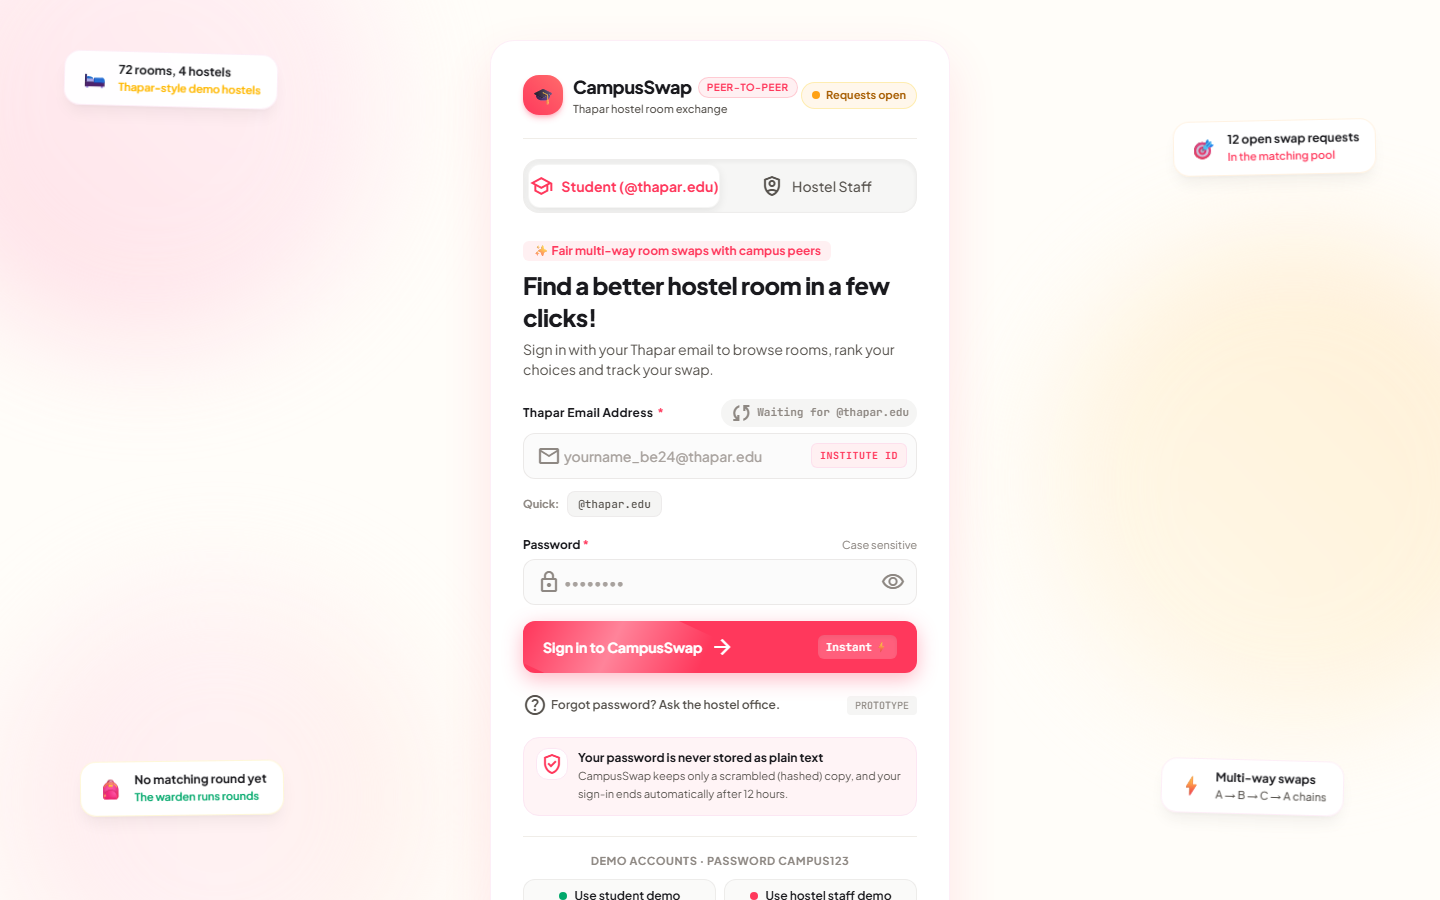
\includegraphics[width=\textwidth,height=0.6\textheight,keepaspectratio]{screen-login.png}
  \caption{Login page with student / hostel staff switch and live pool statistics.}
  \label{fig:login}
\end{figure}

\begin{figure}[H]
  \centering
  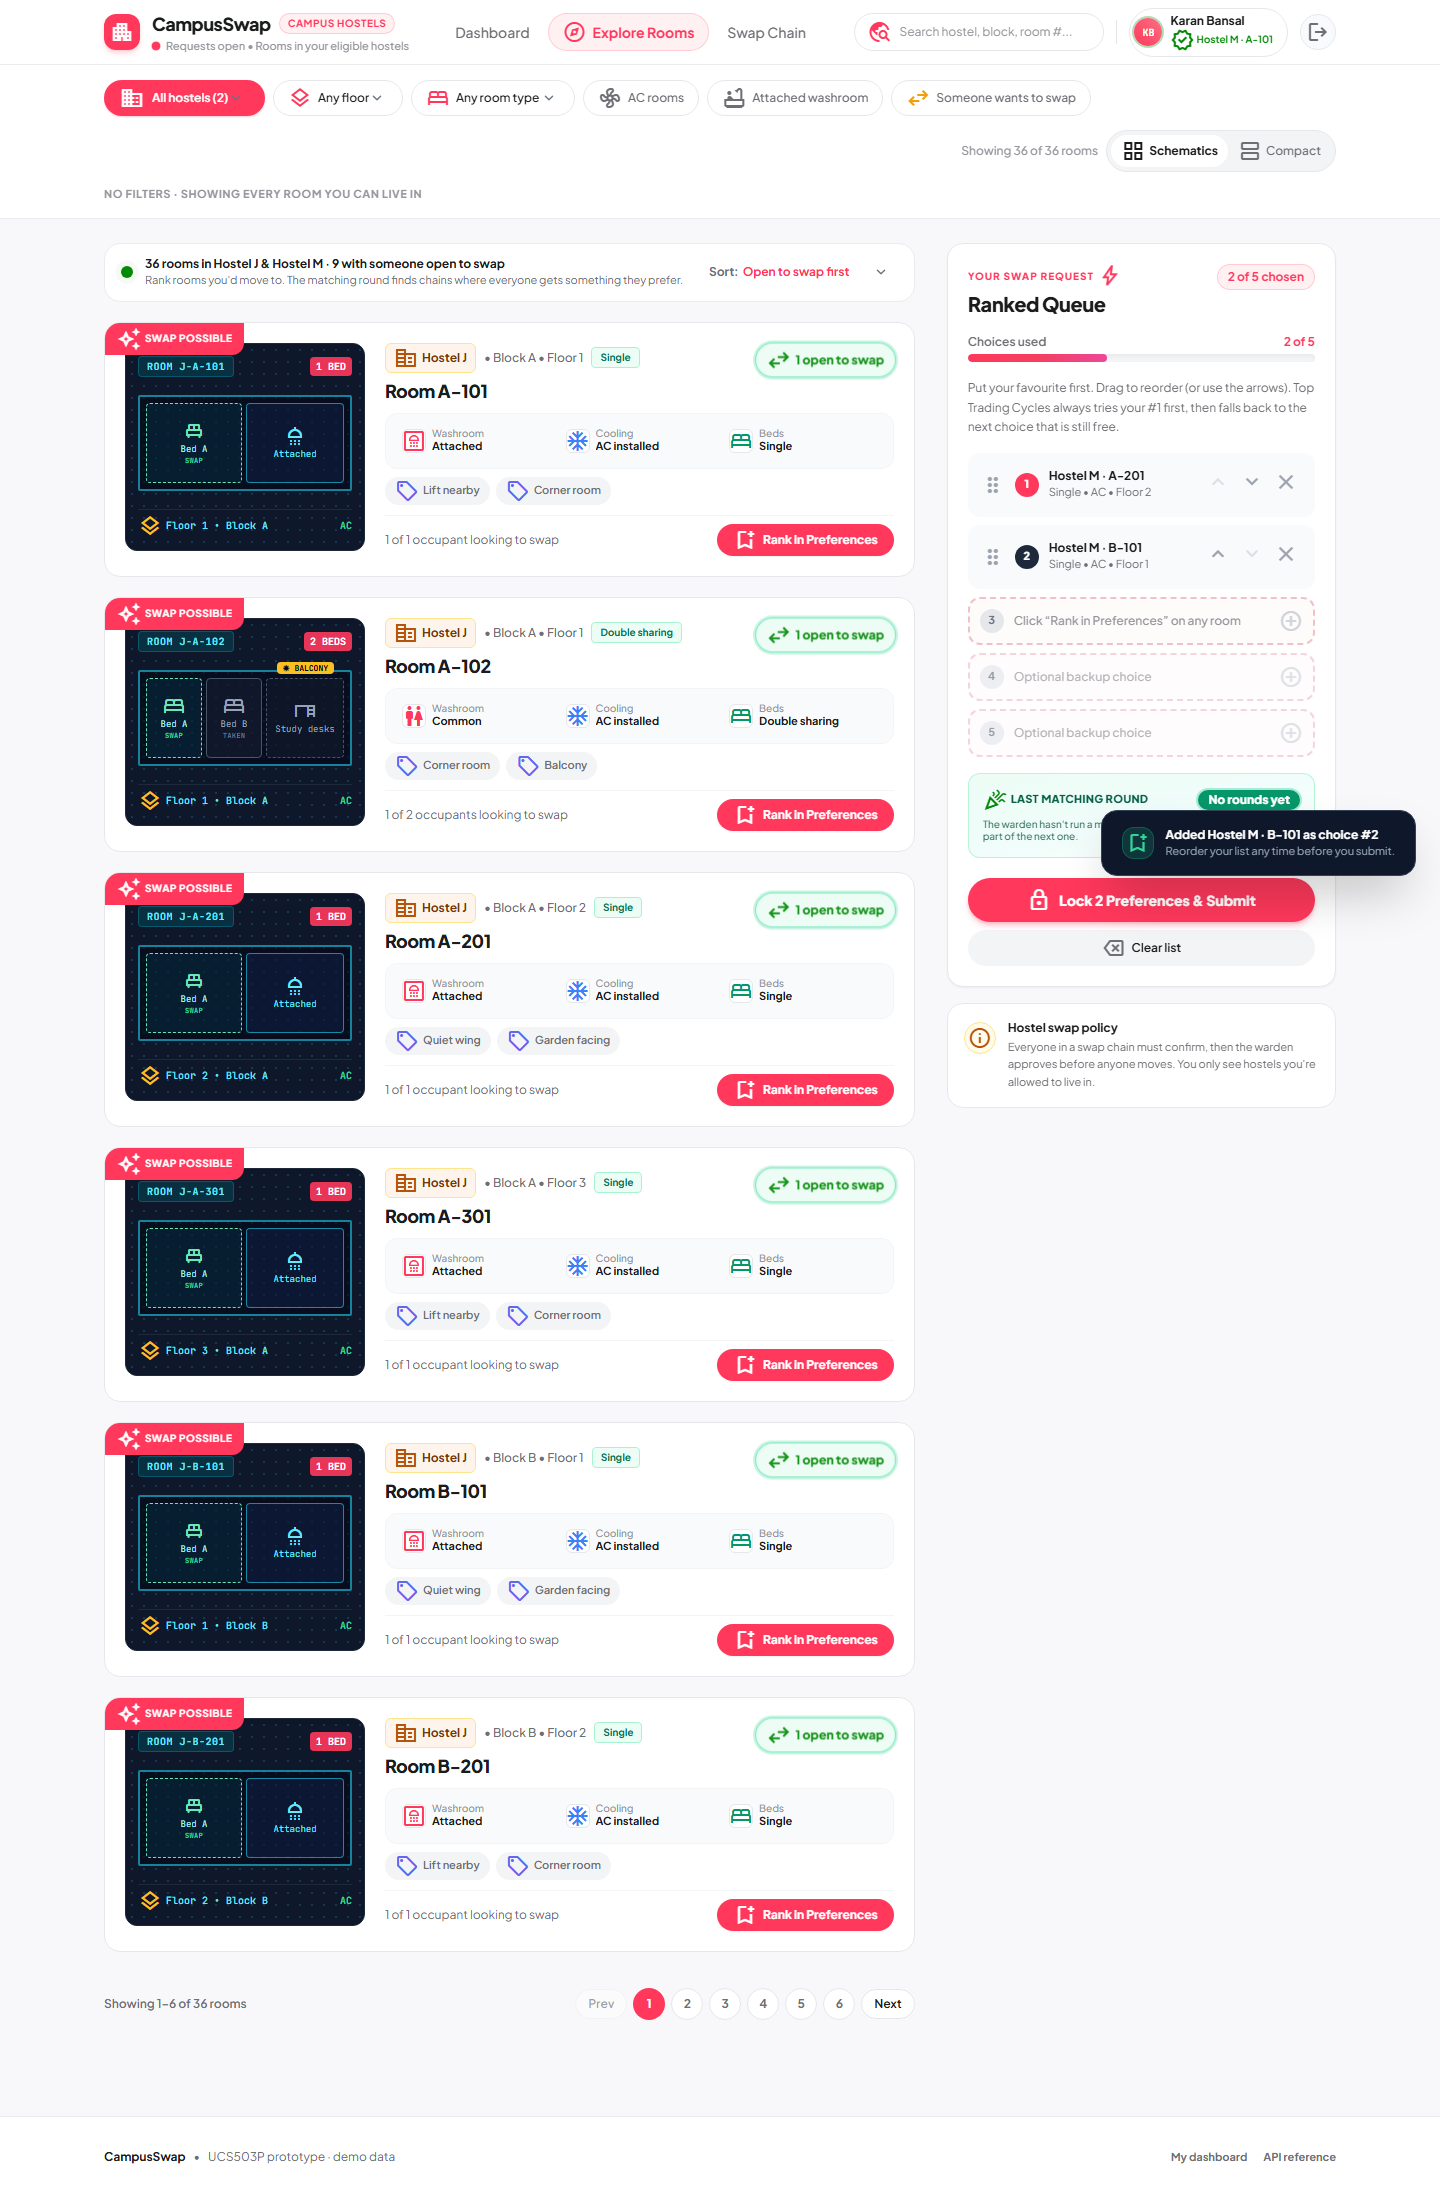
\includegraphics[width=\textwidth,height=0.85\textheight,keepaspectratio]{screen-rooms.png}
  \caption{Feature 1: exploring rooms and building a ranked list.}
  \label{fig:rooms}
\end{figure}

\begin{figure}[H]
  \centering
  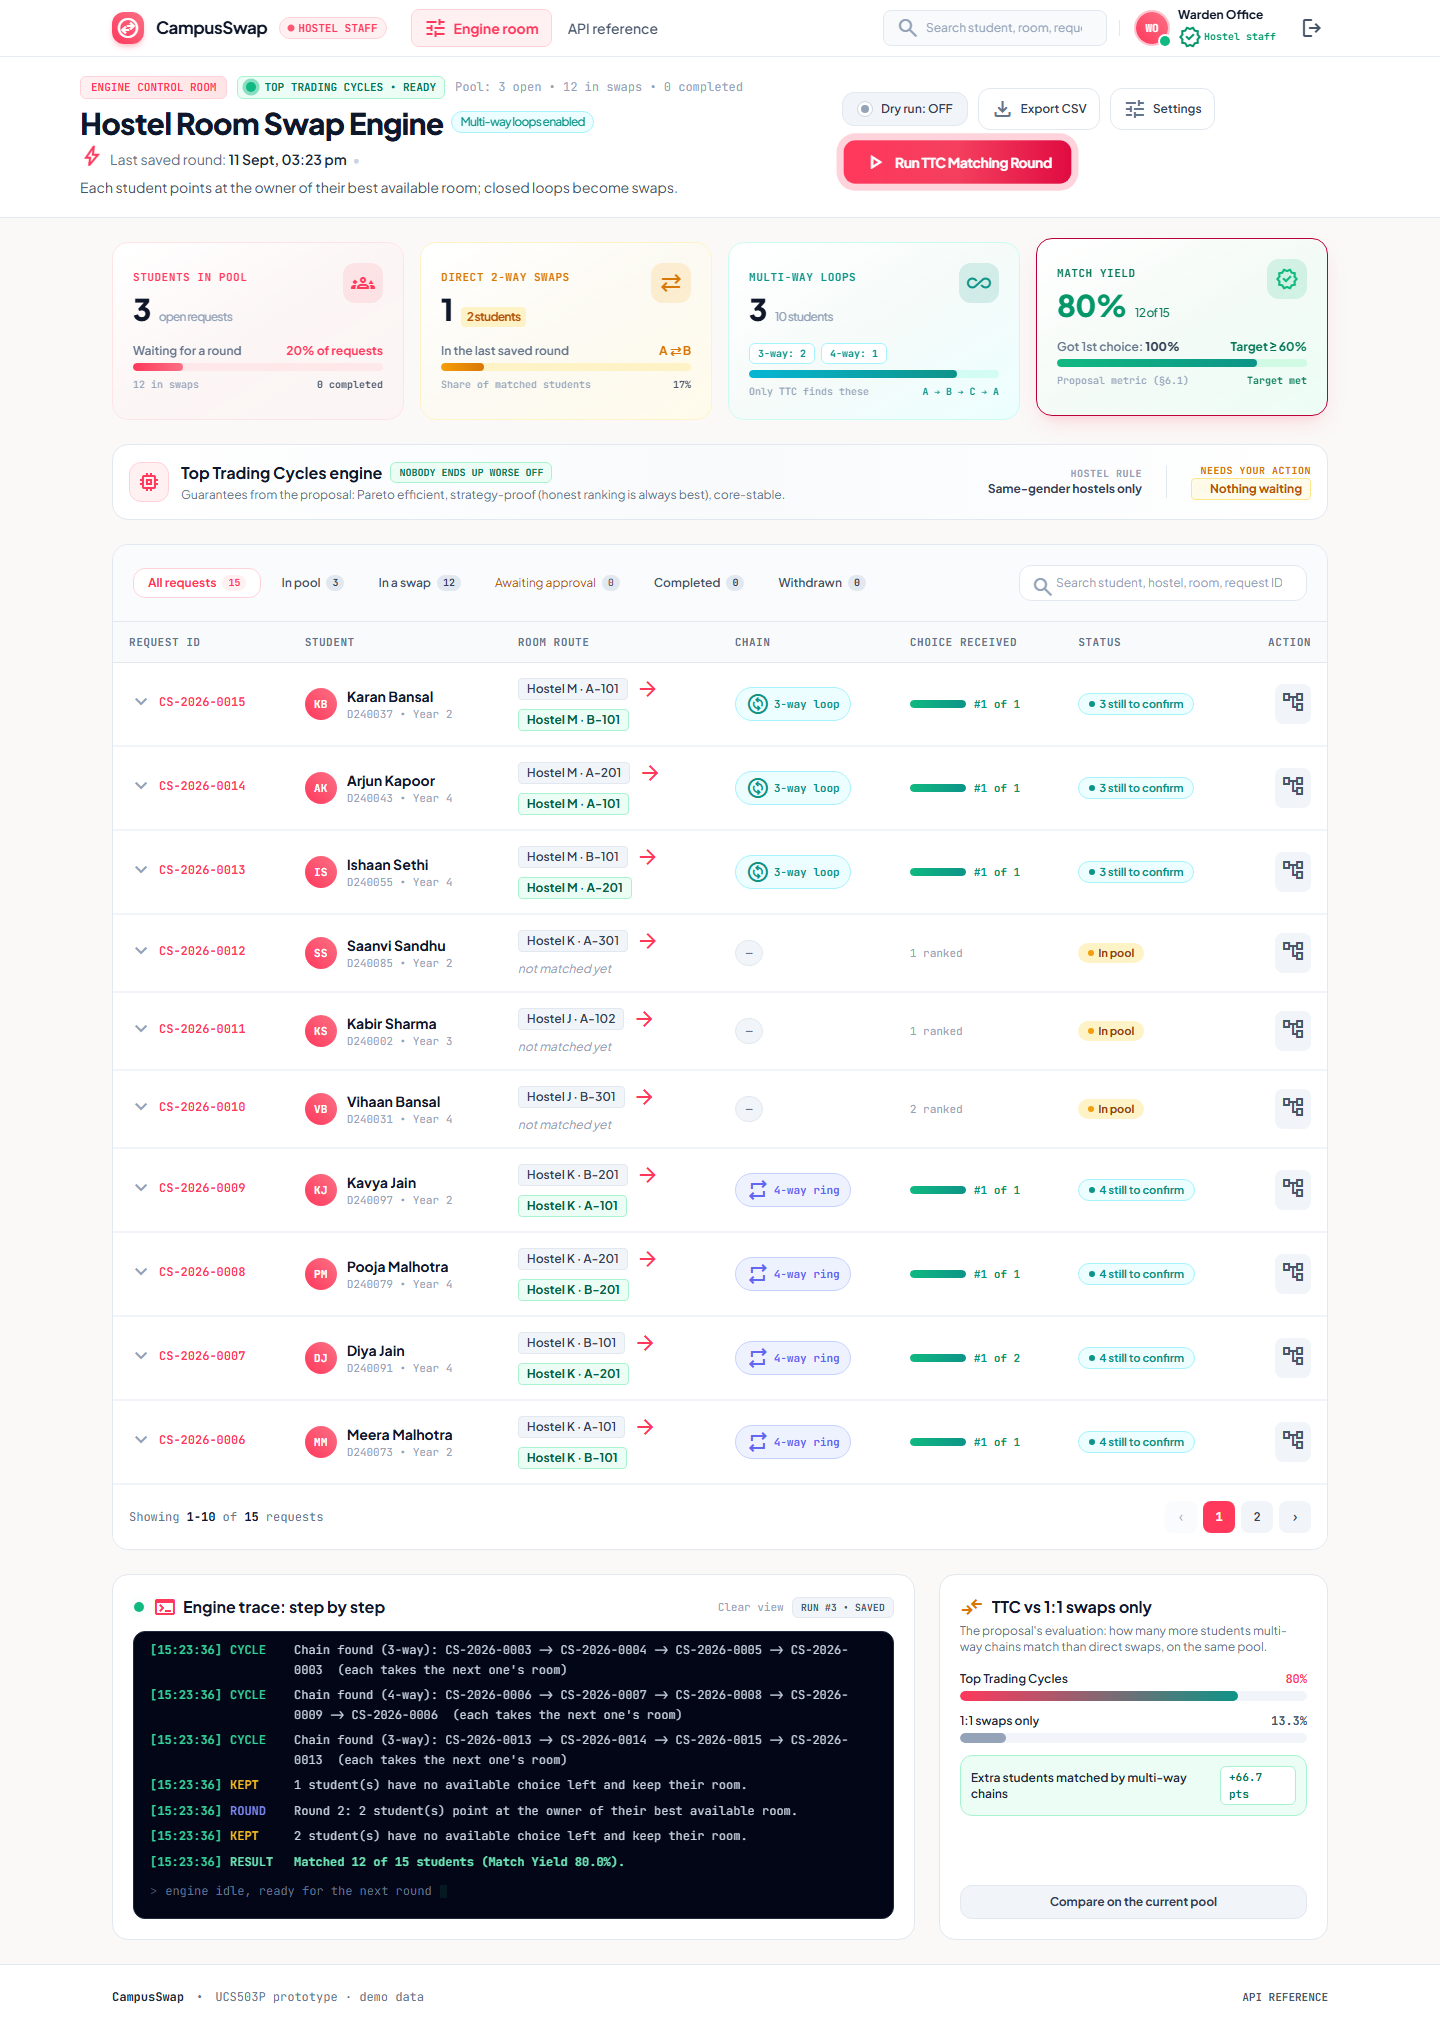
\includegraphics[width=\textwidth,height=0.85\textheight,keepaspectratio]{screen-admin.png}
  \caption{Feature 2: the administrator's engine room after a saved TTC round.}
  \label{fig:admin}
\end{figure}

\begin{figure}[H]
  \centering
  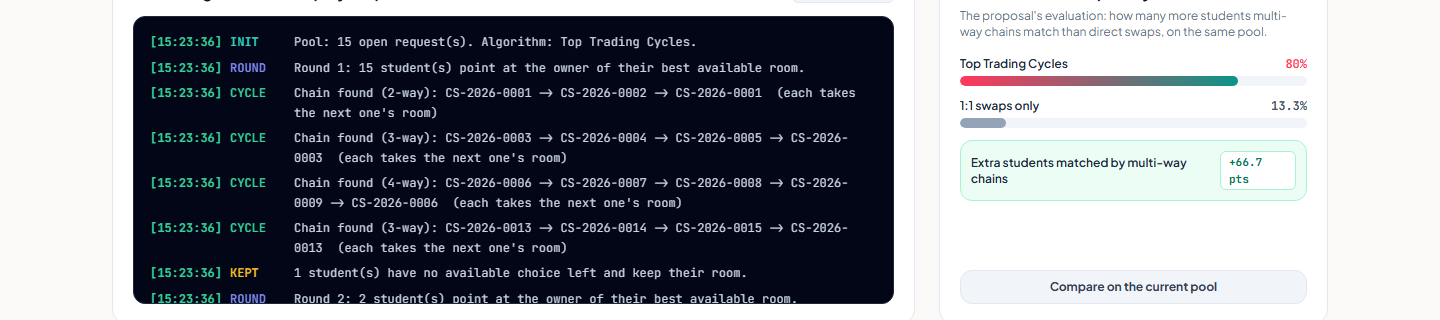
\includegraphics[width=\textwidth]{screen-admin-trace.png}
  \caption{The engine trace explains each TTC round in plain words.}
  \label{fig:trace}
\end{figure}

\begin{figure}[H]
  \centering
  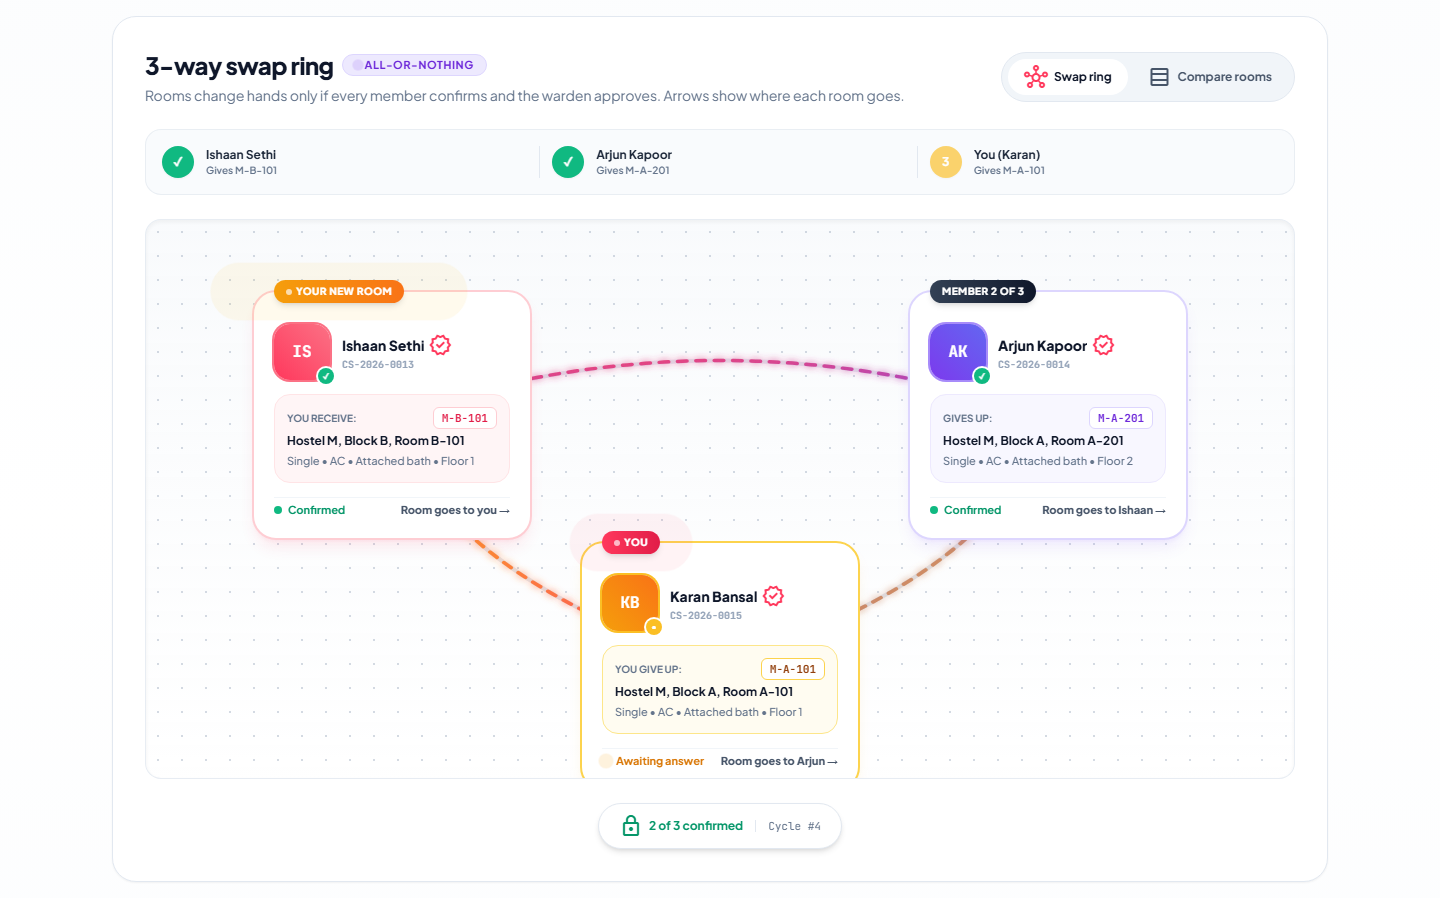
\includegraphics[width=\textwidth,height=0.75\textheight,keepaspectratio]{screen-dashboard-ring.png}
  \caption{Student dashboard: a 3-way swap chain awaiting confirmation.}
  \label{fig:ring}
\end{figure}

\begin{figure}[H]
  \centering
  \begin{subfigure}[t]{0.31\textwidth}
    \centering
    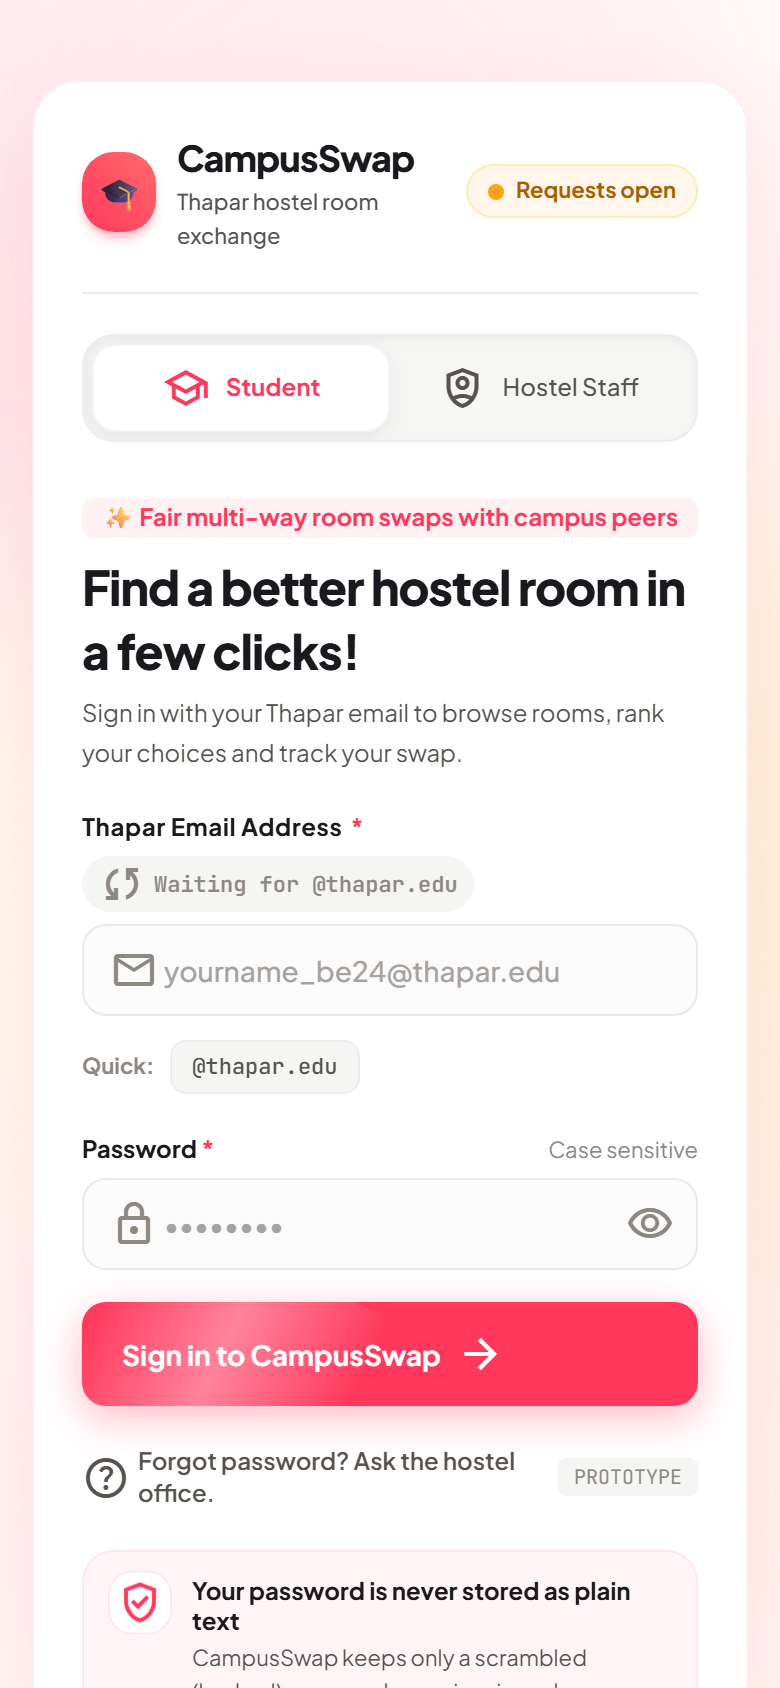
\includegraphics[width=\linewidth]{screen-login-mobile.png}
    \caption{Login}
  \end{subfigure}\hfill
  \begin{subfigure}[t]{0.31\textwidth}
    \centering
    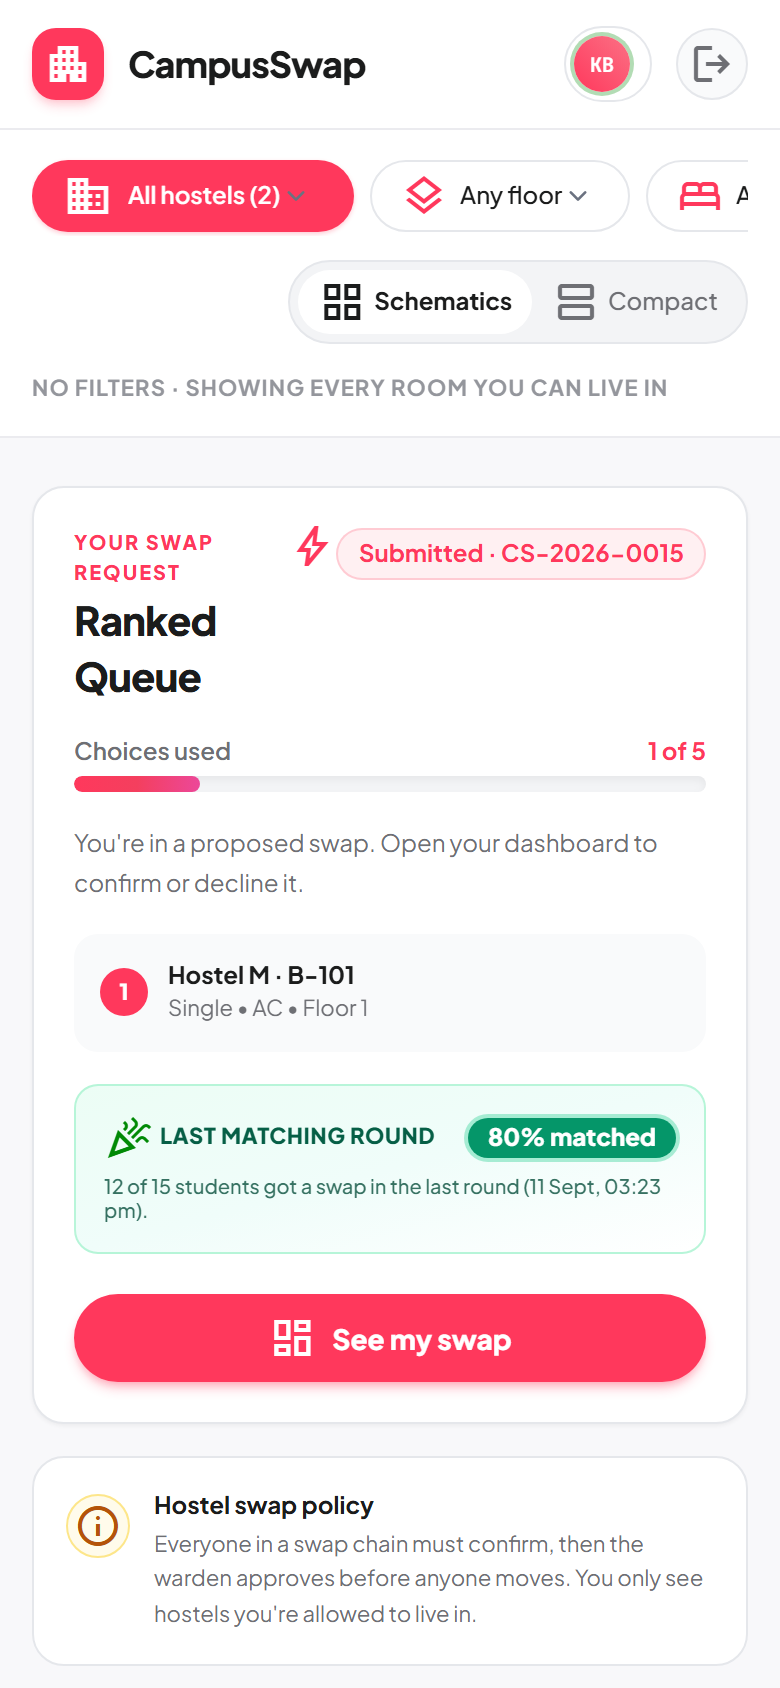
\includegraphics[width=\linewidth]{screen-rooms-mobile.png}
    \caption{Ranked list}
  \end{subfigure}\hfill
  \begin{subfigure}[t]{0.31\textwidth}
    \centering
    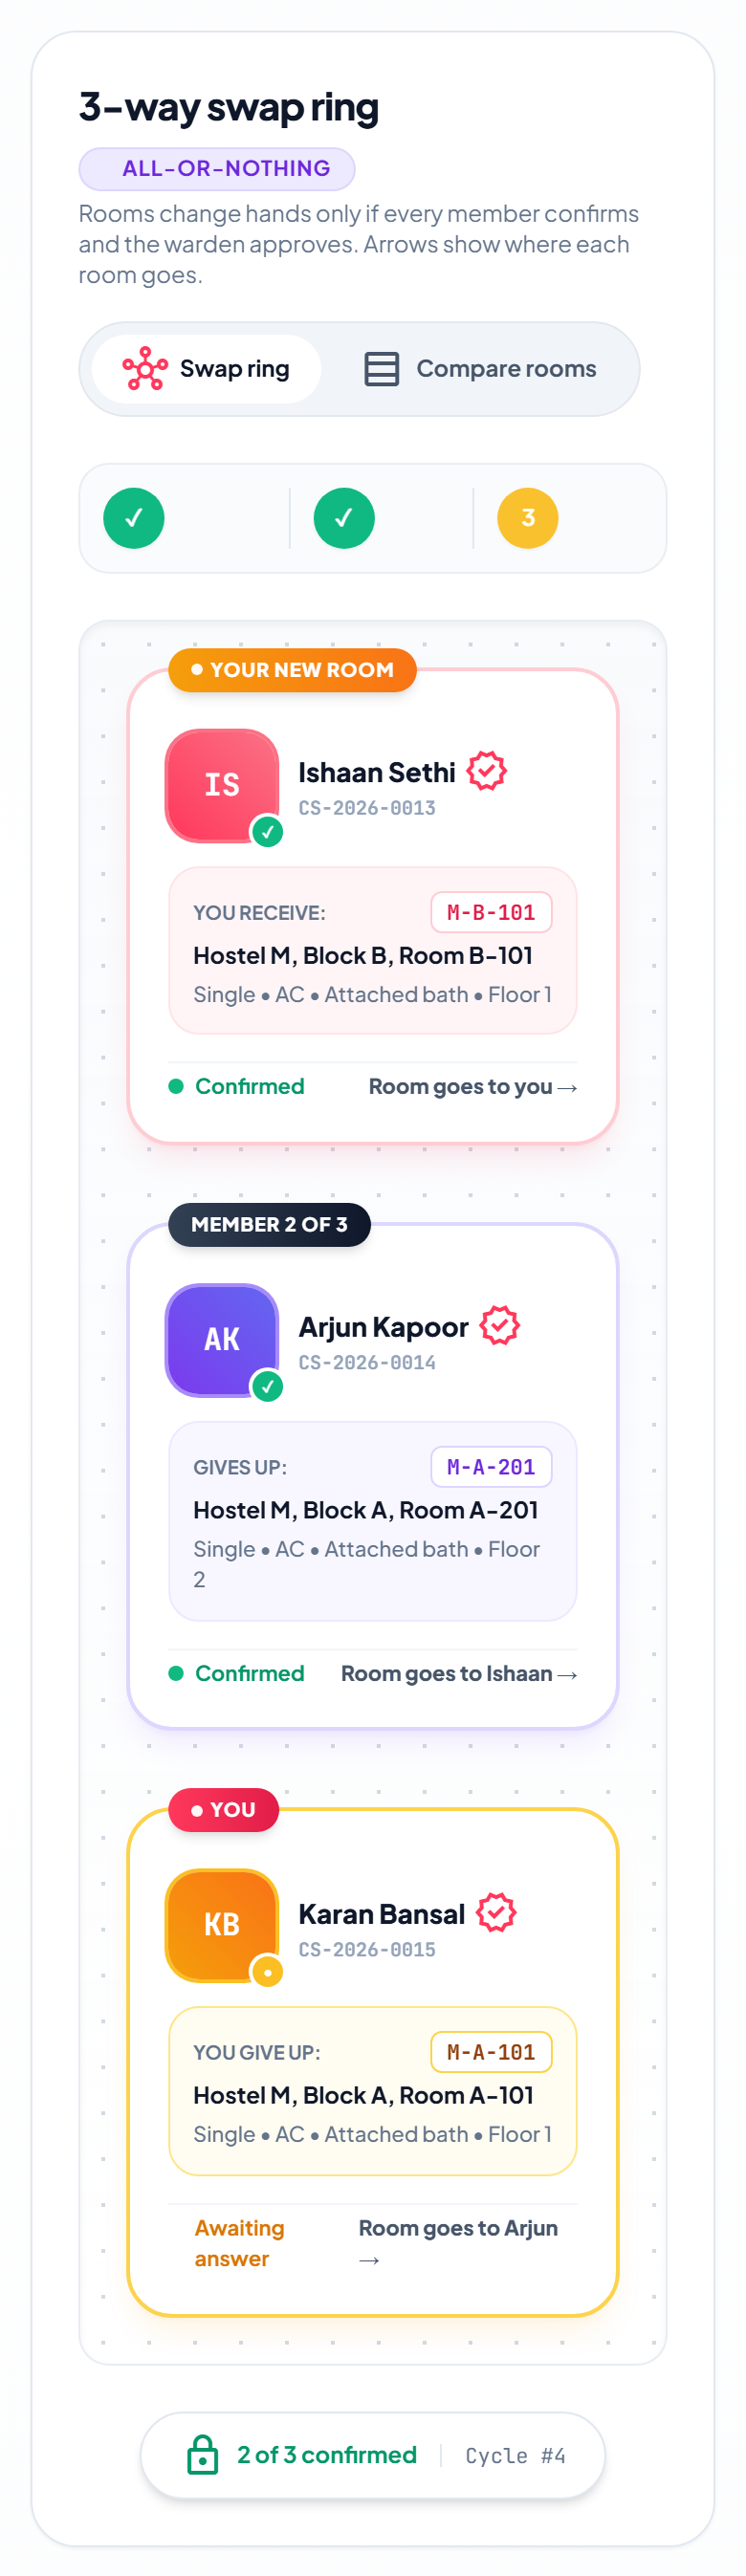
\includegraphics[width=\linewidth,height=0.55\textheight,keepaspectratio]{screen-dashboard-mobile-ring.png}
    \caption{Swap chain}
  \end{subfigure}
  \caption{The same pages on a phone (390\,px wide).}
  \label{fig:mobile}
\end{figure}

\section{Repository, CI and Documentation}

The project follows the course template repository~\cite{campusswaprepo}.
Work is done on a \texttt{prototype} branch and merged into
\texttt{master} through pull requests. A GitHub Actions workflow runs
all tests on every push and pull request, and the course workflow
publishes the MkDocs documentation site, which includes a study guide
for each team role and a question bank.

% =====================================================
\chapter{Testing and Evaluation}
\label{ch:eval}
% =====================================================

\section{Testing}

The suite contains \textbf{90 automated tests}, all passing locally
and in CI. Each test uses a fresh in-memory database and a fixed clock,
so results are repeatable.

\begin{table}[H]
\centering
\begin{tabularx}{\textwidth}{@{}lrL@{}}
\toprule
\textbf{Area} & \textbf{Tests} & \textbf{What is checked} \\
\midrule
Engine (TTC, 1:1, metrics, types) & 28 & 2/3/4-way cycles, fall-back to later choices, double rooms, order independence, 50 random pools obey the guarantees, speed on 2\,000 students \\
Security and demo data & 9 & password hashing, session tokens, seeded data consistency \\
Request rules & 12 & every submission and withdrawal rule \\
Matching service & 9 & known chains on the seeded pool, dry runs change nothing, one run at a time \\
Confirmation workflow & 8 & confirm, decline, deadline expiry, approval moves students \\
Page data & 9 & the data each page receives in every state \\
HTTP API & 15 & login, permissions, readable errors, a full 3-way swap from request to approval \\
\bottomrule
\end{tabularx}
\caption{Automated tests.}
\end{table}

The four pages were additionally driven end to end in a real browser
engine (Microsoft Edge in headless mode): three students submitted,
the warden compared and ran a round, the chain was confirmed and
approved, and the pages reported no script errors.

\section{Match Yield}

\textbf{Demo pool.} The seeded demonstration pool of 12 requests
yields one 2-way, one 3-way and one 4-way chain: MY = 75.0\%, against
16.7\% for 1:1 swaps only. Adding the three live-demo students (a
3-way chain) gives 12 of 15 matched, MY = 80.0\%, against 13.3\% for
1:1 swaps. Both results are asserted by automated tests.

\textbf{Pools of 100 requests.} As the proposal specifies 100 requests,
we generated 200 synthetic pools of 100 students, each owning one seat
and ranking $k$ other seats chosen uniformly at random.

\begin{table}[H]
\centering
\begin{tabular}{@{}lcc@{}}
\toprule
 & \textbf{3 choices each} & \textbf{5 choices each} \\
\midrule
TTC Match Yield, mean (s.d.) & 60.9\% (5.6) & 75.2\% (4.5) \\
TTC Match Yield, range & 45--77\% & 63--87\% \\
1:1 swaps only, mean (s.d.) & 8.4\% (3.9) & 21.6\% (5.2) \\
Chains per pool, mean & 9.2 & 11.5 \\
Share of chains that are 2-way & 16\% & 17\% \\
Longest chain observed & 32 & 33 \\
\bottomrule
\end{tabular}
\caption{Match Yield on 200 random pools of 100 students.}
\label{tab:yield}
\end{table}

TTC meets the target MY~$\geq 60\%$ on average in both settings and
matches three to seven times more students than direct swaps. Only
about one chain in six is a simple 2-way swap, which confirms the
proposal's claim that most feasible exchanges are multi-way.

Two cautions apply. First, uniformly random preferences are a
simplification: real students concentrate on a few popular rooms,
which would lower both yields, so the pilot study remains necessary.
Second, TTC can produce very long chains (up to 33 students here); since
one decline cancels a whole chain, long chains are fragile. Limiting
chain length or re-running TTC on the remaining students after a
decline are candidate improvements.

\section{Performance}

\begin{table}[H]
\centering
\begin{tabular}{@{}rr@{}}
\toprule
\textbf{Students} & \textbf{TTC time (best of 3)} \\
\midrule
100 & 0.2 ms \\
1\,000 & 4.8 ms \\
2\,000 & 15.4 ms \\
5\,000 & 58.0 ms \\
\bottomrule
\end{tabular}
\caption{TTC running time with five choices per student (Python 3.12, laptop).}
\end{table}

Even 5\,000 students are matched in well under a tenth of a second,
so running a round inside the web request is adequate for a campus.

\section{Objectives Review}

\begin{table}[H]
\centering
\begin{tabularx}{\textwidth}{@{}llL@{}}
\toprule
\textbf{Objective} & \textbf{Status} & \textbf{Evidence} \\
\midrule
O1 Data model & Met (partly) & 11 tables with integrity constraints; a formal migration tool is not yet used \\
O2 Student module & Met & login, room browser, ranked requests; 12 rule tests \\
O3 Matching engine & Met & TTC with 28 engine tests \\
O4 Dashboards and CI & Met & student dashboard, admin console, tests on every push \\
O5 Evaluation & Met on synthetic data & MY 75.2\% (5 choices) and 60.9\% (3 choices) on 100-student pools \\
Phase 2: confirmation & Delivered early & multi-party confirm/decline with 48-hour deadline \\
Phase 2: warden portal & Partly & approval, CSV export, audit log; no PDF form yet \\
\bottomrule
\end{tabularx}
\caption{Objectives and their status at the prototype stage.}
\end{table}

\section{Deviations from the Proposal}

\begin{itemize}
  \item \textbf{No background worker.} Rounds run inside the web
    request; the measured running times make a job queue unnecessary at
    this scale.
  \item \textbf{No scheduler.} Overdue chains are dissolved whenever a
    round runs or a member answers, instead of by a timer.
  \item \textbf{E-mail and password login} instead of the institute
    login, which requires university approval.
  \item \textbf{SQLite} rather than a database server, to keep the
    prototype self-contained; SQLAlchemy allows switching later.
\end{itemize}

% =====================================================
\chapter{Conclusion and Future Work}
% =====================================================

\section{Summary}

The prototype meets the Phase~1 success definition: it accepts ranked
requests, stores them, runs a Top Trading Cycles match and shows the
result to students and staff. It also delivers the multi-party
confirmation workflow planned for Phase~2, backed by 90 automated tests
and a published documentation site.

\section{Key Findings}

\begin{itemize}
  \item Multi-way exchange matters: on 100-student pools TTC matched
    75.2\% of students against 21.6\% for direct swaps (five choices).
  \item Keeping the algorithm separate from web and database code made
    it straightforward to test thoroughly and to measure.
  \item Long chains are the main practical risk, because one decline
    cancels the whole chain.
\end{itemize}

\section{Future Work}

\begin{enumerate}
  \item Pilot with 20--40 students from one hostel wing to measure real
    Match Yield, time to approval and confirmation drop-off.
  \item Notifications when a chain is found, and the PDF sign-off form.
  \item Handling fragile long chains (length limits or re-matching after
    a decline).
  \item Ranking by room type or floor, not only specific rooms.
  \item The faculty slot-exchange module, reusing the same engine.
  \item Institute single sign-on and deployment to a hosted server.
\end{enumerate}

\section{Team Roles}

\begin{table}[H]
\centering
\begin{tabularx}{\textwidth}{@{}lL@{}}
\toprule
\textbf{Role} & \textbf{Responsibility} \\
\midrule
P1 Frontend & the four pages, JavaScript modules and styling build \\
P2 Backend and login & API routes, sessions, request and confirmation rules \\
P3 Matching engine & TTC, the 1:1 baseline, Match Yield and engine tests \\
P4 Data, diagrams and delivery & data model, demo data, UML diagrams, CI, documentation and this report \\
\bottomrule
\end{tabularx}
\caption{Team roles; each member records their role in their weekly journal.}
\end{table}

% ===== BIBLIOGRAPHY =====

\printbibliography[heading=bibintoc]

\end{document}
